\documentclass[oneside]{book}\twocolumn
\usepackage[utf8]{inputenc}
\usepackage{pgfplots}
\pgfplotsset{compat=1.15}
\usepackage{mathrsfs}
\usetikzlibrary{arrows}
\usepackage{amsmath}
\usepackage{tikz}
\usepackage{wrapfig}
\usepackage{parskip}
\usepackage[most]{tcolorbox}
\usepackage{amssymb}
\usepackage{amsthm}
\usepackage[margin=0.7in]{geometry}
\usepackage{mathtools}
\usepackage{caption}
\usepackage{float}
\usepackage{enumitem}

\newtheorem{theorem}{Theorem}
\newtheorem{definition}[theorem]{Definition}
\newtheorem{claim}[theorem]{Claim}
\newtheorem{proposition}[theorem]{Proposition}
\newtheorem{lemma}[theorem]{Lemma}
\newtheorem{corollary}[theorem]{Corollary}
\newtheorem{conjecture}[theorem]{Conjecture}
\newtheorem*{observation}{Observation}
\newtheorem*{example}{Example}
\newtheorem*{remark}{Remark}

\usepackage{physics}
\usepackage{amsmath}
\usepackage{tikz}
\usepackage{mathdots}
\usepackage{yhmath}
\usepackage{cancel}
\usepackage{color}
\usepackage{siunitx}
\usepackage{array}
\usepackage{multirow}
\usepackage{amssymb}
\usepackage{gensymb}
\usepackage{tabularx}
\usepackage{extarrows}
\usepackage{booktabs}
\usetikzlibrary{fadings}
\usetikzlibrary{patterns}
\usetikzlibrary{shadows.blur}
\usetikzlibrary{shapes}




\tcbset{mytitle/.style={title={Question~\thetcbcounter\ifstrempty{#1}{}{: #1}}}}
\newtcolorbox[auto counter, number within=chapter, number freestyle={\noexpand\thechapter.\noexpand\arabic{\tcbcounter}}]{question}[1][]{%
    enhanced,
    breakable,
    fonttitle=\bfseries,
    mytitle={},
    #1
}


\title{Lecture Notes for Graphs and Surfaces}
\author{Aakash Ghosh }
\date{Instructor: Prof. Somnath Basu}
\begin{document}
\maketitle
\tableofcontents


\chapter{What to expect}
First we shall see some theorems and examples and get to know the terms on an intuitive sense. The formal definitions of everything will be provided down the line(probably).
\section{Four vertex theorem}
\begin{theorem}[Four Vertex Theorem]
The curvature of a simple closed smooth curve has at least 2 local minima and two local maxima.
\end{theorem}
\textbf{[Planar] Curve:} A curve is a map $f$ from $\mathbb R\to\mathbb R^2$. Note: other types of curves exists. For example, a space curve is a map from $\mathbb R\to\mathbb R^3$.\\
\textbf{Smooth:} Smooth implies that the $k^{th}$ derivative of $f$ defined in the previous section exists and is continuous for all $k\in\mathbb N$.\\
\textbf{Closed:} Intuitively, a closed curve has the same starting and ending point. We define $f:[0,c]\to\mathbb R^2$ as closed if $f(0)=f(c)$. If we want to define it according to the definition we gave earlier, we say $f$ is periodic. This implies for every $p\in\mathbb R$, $f(p+c)=f(p)$. The smallest such $c$ is known as the period of the function. We can also view this in an geometric way: A closed curve is a mapping of $S^1$ to $\mathbb R^2$($S^1$ is the unit circle in $\mathbb R^2$ plane). Let $e^{i\theta}$ be a point on $S^1$. Then a closed curve is a mapping $\Tilde{f}:S^1\to \mathbb{R}^2$. Now we can of course relate $\Tilde{f}$ and $f$ in a very natural way: $\Tilde{f}(e^{i\theta})=f(\frac{c}{2\pi}\theta)$(This result comes from the fact that the parameters which define $S^1$, i.e $\sin\theta$ and $\cos\theta$ are periodic in nature).\\
\textbf{Simple :}Intuitively, a simple curve is a curve which doesn't cross or touch itself. Therefore, if you zoom close enough at any point, it looks like a regular arc. mathematically we need $\Tilde{f}$ to be injective or one-one.


\tikzset{every picture/.style={line width=0.75pt}} %set default line width to 0.75pt        

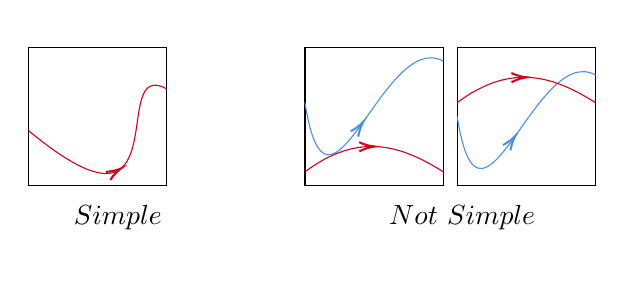
\begin{tikzpicture}[x=0.5pt,y=0.5pt,yscale=-1,xscale=1]
%uncomment if require: \path (0,300); %set diagram left start at 0, and has height of 300

%Shape: Rectangle [id:dp48033389218446143] 
\draw   (50,100) -- (150,100) -- (150,200) -- (50,200) -- cycle ;
%Shape: Rectangle [id:dp4215438801436513] 
\draw   (250,100) -- (350,100) -- (350,200) -- (250,200) -- cycle ;
%Shape: Rectangle [id:dp18460370937318105] 
\draw   (360,100) -- (460,100) -- (460,200) -- (360,200) -- cycle ;
%Curve Lines [id:da511310320695898] 
\draw [color={rgb, 255:red, 208; green, 2; blue, 27 }  ,draw opacity=1 ]   (50,160) .. controls (162.2,253) and (106.6,106.2) .. (150,130) ;
\draw [shift={(117.17,187.48)}, rotate = 150.29] [color={rgb, 255:red, 208; green, 2; blue, 27 }  ,draw opacity=1 ][line width=0.75]    (10.93,-3.29) .. controls (6.95,-1.4) and (3.31,-0.3) .. (0,0) .. controls (3.31,0.3) and (6.95,1.4) .. (10.93,3.29)   ;
%Curve Lines [id:da8342244921465348] 
\draw [color={rgb, 255:red, 74; green, 144; blue, 226 }  ,draw opacity=1 ]   (250,140) .. controls (267,248.2) and (306.6,86.2) .. (350,110) ;
\draw [shift={(292.21,153.72)}, rotate = 125.98] [color={rgb, 255:red, 74; green, 144; blue, 226 }  ,draw opacity=1 ][line width=0.75]    (10.93,-3.29) .. controls (6.95,-1.4) and (3.31,-0.3) .. (0,0) .. controls (3.31,0.3) and (6.95,1.4) .. (10.93,3.29)   ;
%Curve Lines [id:da35976819210964917] 
\draw [color={rgb, 255:red, 208; green, 2; blue, 27 }  ,draw opacity=1 ]   (250,190) .. controls (290,160) and (321,171.8) .. (350,190) ;
\draw [shift={(300.17,171.69)}, rotate = 178.96] [color={rgb, 255:red, 208; green, 2; blue, 27 }  ,draw opacity=1 ][line width=0.75]    (10.93,-3.29) .. controls (6.95,-1.4) and (3.31,-0.3) .. (0,0) .. controls (3.31,0.3) and (6.95,1.4) .. (10.93,3.29)   ;
%Curve Lines [id:da6101296278737137] 
\draw [color={rgb, 255:red, 74; green, 144; blue, 226 }  ,draw opacity=1 ]   (360,150) .. controls (377,258.2) and (416.6,96.2) .. (460,120) ;
\draw [shift={(402.21,163.72)}, rotate = 125.98] [color={rgb, 255:red, 74; green, 144; blue, 226 }  ,draw opacity=1 ][line width=0.75]    (10.93,-3.29) .. controls (6.95,-1.4) and (3.31,-0.3) .. (0,0) .. controls (3.31,0.3) and (6.95,1.4) .. (10.93,3.29)   ;
%Curve Lines [id:da6787942491941835] 
\draw [color={rgb, 255:red, 208; green, 2; blue, 27 }  ,draw opacity=1 ]   (360,140) .. controls (400,110) and (431,121.8) .. (460,140) ;
\draw [shift={(410.17,121.69)}, rotate = 178.96] [color={rgb, 255:red, 208; green, 2; blue, 27 }  ,draw opacity=1 ][line width=0.75]    (10.93,-3.29) .. controls (6.95,-1.4) and (3.31,-0.3) .. (0,0) .. controls (3.31,0.3) and (6.95,1.4) .. (10.93,3.29)   ;

% Text Node
\draw (81,212.4) node [anchor=north west][inner sep=0.75pt]    {$Simple$};
% Text Node
\draw (309,212.4) node [anchor=north west][inner sep=0.75pt]    {$Not\ Simple$};


\end{tikzpicture}

\textbf{Curvature :}Curvature is basically a function from the points of the curve to $\mathbb R$. Specifically $\mathcal{K}:\mathbb{R}^2\to\mathbb{R}$, where $\mathcal{K}(\Tilde{f}(e^{i\theta}))$ gives the inverse of the radius of the circle with the best fit at the point $\Tilde{f}(e^{i\theta})$. Now this circle of best fit needs to be defined with some care. for one the the point and the circle drawn share the same normal and tangent.
\begin{figure}[!htb]
    
\centering
\tikzset{every picture/.style={line width=0.75pt}} %set default line width to 0.75pt        

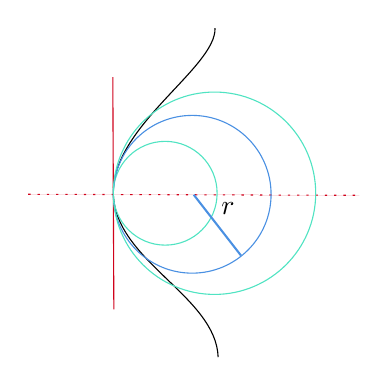
\begin{tikzpicture}[x=0.75pt,y=0.75pt,yscale=-1,xscale=1]
%uncomment if require: \path (0,300); %set diagram left start at 0, and has height of 300

%Curve Lines [id:da8990808912090099] 
\draw    (161,218.75) .. controls (160,189.25) and (111,172.25) .. (110.5,139.75) .. controls (110,107.25) and (160,79.25) .. (159.5,60.25) ;
%Straight Lines [id:da5329665639527169] 
\draw [color={rgb, 255:red, 208; green, 2; blue, 27 }  ,draw opacity=1 ]   (110.25,83.75) -- (110.75,195.75) ;
%Straight Lines [id:da996193084348262] 
\draw [color={rgb, 255:red, 208; green, 2; blue, 27 }  ,draw opacity=1 ][fill={rgb, 255:red, 208; green, 2; blue, 27 }  ,fill opacity=1 ] [dash pattern={on 0.84pt off 2.51pt}]  (69.5,140.25) -- (229,140.75) ;
%Shape: Circle [id:dp671885589792057] 
\draw  [color={rgb, 255:red, 80; green, 227; blue, 194 }  ,draw opacity=1 ] (110.5,139.75) .. controls (110.5,125.94) and (121.69,114.75) .. (135.5,114.75) .. controls (149.31,114.75) and (160.5,125.94) .. (160.5,139.75) .. controls (160.5,153.56) and (149.31,164.75) .. (135.5,164.75) .. controls (121.69,164.75) and (110.5,153.56) .. (110.5,139.75) -- cycle ;
%Shape: Circle [id:dp916983786523555] 
\draw  [color={rgb, 255:red, 74; green, 144; blue, 226 }  ,draw opacity=1 ] (110.5,140.25) .. controls (110.5,119.26) and (127.51,102.25) .. (148.5,102.25) .. controls (169.49,102.25) and (186.5,119.26) .. (186.5,140.25) .. controls (186.5,161.24) and (169.49,178.25) .. (148.5,178.25) .. controls (127.51,178.25) and (110.5,161.24) .. (110.5,140.25) -- cycle ;
%Shape: Circle [id:dp7636897615627564] 
\draw  [color={rgb, 255:red, 80; green, 227; blue, 194 }  ,draw opacity=1 ] (110.5,139.75) .. controls (110.5,112.83) and (132.33,91) .. (159.25,91) .. controls (186.17,91) and (208,112.83) .. (208,139.75) .. controls (208,166.67) and (186.17,188.5) .. (159.25,188.5) .. controls (132.33,188.5) and (110.5,166.67) .. (110.5,139.75) -- cycle ;
%Straight Lines [id:da3292244417302711] 
\draw [color={rgb, 255:red, 74; green, 144; blue, 226 }  ,draw opacity=1 ][line width=0.75]    (149.25,140.5) -- (172,169.75) ;

% Text Node
\draw (161.25,143.15) node [anchor=north west][inner sep=0.75pt]    {$r$};


\end{tikzpicture}

    \caption{The red lines are common normal and common tangent. Note, the circle of medium size somehow seems to be a better fit than the others. So the radius of curvature at that point is $\frac{1}{r}$}
    \label{fig:my_label}
\end{figure}
One way to drive this concept home for planar curve is to consider the following process: take any three points $t_1,t_2,t_3$ around $t$. Draw the circumcircle of those points. the radius of curvature will be the radius of the circle formed when $\lim{t_1,t_2,t_3\to t}$


\tikzset{every picture/.style={line width=0.75pt}} %set default line width to 0.75pt        

\begin{tikzpicture}[x=0.75pt,y=0.75pt,yscale=-1,xscale=1]
%uncomment if require: \path (0,300); %set diagram left start at 0, and has height of 300

%Curve Lines [id:da026905970078967] 
\draw    (51.43,191.95) .. controls (224.17,191.05) and (197.6,149.86) .. (219.84,149.86) .. controls (242.09,149.86) and (222.32,191.05) .. (417,192.24) ;
%Shape: Ellipse [id:dp8371132730905899] 
\draw  [color={rgb, 255:red, 208; green, 2; blue, 27 }  ,draw opacity=1 ] (176.89,208.36) .. controls (176.89,179.51) and (201.1,156.13) .. (230.97,156.13) .. controls (260.84,156.13) and (285.05,179.51) .. (285.05,208.36) .. controls (285.05,237.21) and (260.84,260.6) .. (230.97,260.6) .. controls (201.1,260.6) and (176.89,237.21) .. (176.89,208.36) -- cycle ;

% Text Node
\draw (175.66,150.49) node [anchor=north west][inner sep=0.75pt]    {$t_{1}$};
% Text Node
\draw (232.86,135.29) node [anchor=north west][inner sep=0.75pt]    {$t_{2}$};
% Text Node
\draw (276.46,158.49) node [anchor=north west][inner sep=0.75pt]    {$t_{3}$};
% Text Node
\draw (214,131.6) node [anchor=north west][inner sep=0.75pt]    {$t$};


\end{tikzpicture}
The figure above shows the process. While this is nice way to view things, it is has it's own set of problems: How do we know that a limit exists? More over in higher dimensional spaces, the plane in which the circle lies will also change with the points that are being considered. Nevertheless it's good enough for a naive mental picture. The rest of the theorem now makes sense. 














\section{Fary-Milnor theorem}
\begin{theorem}[Fary-Milnor theorem]
If the total absolute curvature of a knot $K$ is at most $4\pi$, then $K$ is an unknot.
\end{theorem}
\textbf{Knot :}A knot is a simple curve in 3-space. 
\textbf{Total absolute curvature :}What it says. We can't of course take an infinite sum for all the points so we integrate. 
\begin{align}
    S=\int_\mathcal{S}\left|\mathcal{K}(s)\right|ds
\end{align}
\textbf{Unknot :}A unknot is a knot which can be deformed to a circle.
\begin{figure}[!htb]
    \centering
    \includegraphics[width=0.45\textwidth]{The_two_trefoil_knots.png}
    \caption{The two trefoil knots. They are not unknots(Copied from Wikipedia)}
    \label{fig:my_label}
\end{figure}
\section{Hirsch-Smale Theory}
\begin{theorem}[Hirsch-Smale Theory]
Any two immersed loop in $\mathbb R^2$ are isotopic if and only if the winding numbers match.
\end{theorem}
\textbf{Loop:} A loop is a closed curve\\
\textbf{Immersed:} $f:\mathbb R\to\mathbb R^k$ is said to be immersed if $f'(t)$ is never zero. Note, the drawing of any curve is the trace of a curve: It does not represent the curve itself.\\
\textbf{Isotopic:} This means they are the same. It is what isomorphism is for groups and homeomorphism is for topologies. But when are two loops isotopic?
\begin{figure}[!htb]
    \centering
    

\tikzset{every picture/.style={line width=0.75pt}} %set default line width to 0.75pt        

\begin{tikzpicture}[x=0.5pt,y=0.5pt,yscale=-1,xscale=1]
%uncomment if require: \path (0,300); %set diagram left start at 0, and has height of 300

%Shape: Circle [id:dp3439595731687489] 
\draw   (20,100) .. controls (20,55.82) and (55.82,20) .. (100,20) .. controls (144.18,20) and (180,55.82) .. (180,100) .. controls (180,144.18) and (144.18,180) .. (100,180) .. controls (55.82,180) and (20,144.18) .. (20,100) -- cycle ;
%Shape: Triangle [id:dp1382493260916383] 
\draw  [fill={rgb, 255:red, 0; green, 0; blue, 0 }  ,fill opacity=1 ] (135.32,28.16) -- (126,28.81) -- (132.5,19.25) -- cycle ;
%Curve Lines [id:da9272590436110197] 
\draw    (236,40.5) .. controls (276,10.5) and (368,-0.25) .. (336,40.5) .. controls (304,81.25) and (454,85.25) .. (375.5,140.25) .. controls (297,195.25) and (180,204.25) .. (255,121.25) .. controls (330,38.25) and (211,65.5) .. (236,40.5) -- cycle ;
\draw [shift={(298.5,15.66)}, rotate = 169.09] [fill={rgb, 255:red, 0; green, 0; blue, 0 }  ][line width=0.08]  [draw opacity=0] (8.93,-4.29) -- (0,0) -- (8.93,4.29) -- cycle    ;
\draw [shift={(377.38,87.39)}, rotate = 209.14] [fill={rgb, 255:red, 0; green, 0; blue, 0 }  ][line width=0.08]  [draw opacity=0] (8.93,-4.29) -- (0,0) -- (8.93,4.29) -- cycle    ;
\draw [shift={(277.57,181.23)}, rotate = 350.42] [fill={rgb, 255:red, 0; green, 0; blue, 0 }  ][line width=0.08]  [draw opacity=0] (8.93,-4.29) -- (0,0) -- (8.93,4.29) -- cycle    ;
\draw [shift={(278.02,69.26)}, rotate = 70.96] [fill={rgb, 255:red, 0; green, 0; blue, 0 }  ][line width=0.08]  [draw opacity=0] (8.93,-4.29) -- (0,0) -- (8.93,4.29) -- cycle    ;

% Text Node
\draw (93,212.4) node [anchor=north west][inner sep=0.75pt]    {$\gamma $};
% Text Node
\draw (308.5,210.9) node [anchor=north west][inner sep=0.75pt]    {$\eta $};


\end{tikzpicture}



    \caption{Two isotopic curves: The second one can be "straightened out" into the first one}
    \label{fig:my_label}
\end{figure}
But how to check this? We construct a $f$ which deforms $\eta$ to $\gamma$. But note: merely the presence of such a function is not enough. This would imply any two loops are isotopic. We furthermore require at any instant of the transformation, the resulting curve is  immersed. Now we shall talk a bit about the function. Let $H:S^1\times I\to\mathbb R^2$, where $I=[0,1]$. Now note that the set $S^1\times I\to\mathbb R^2$ looks like a cylinder. $S^1$ represents the base, $I$ represents the height. We think of moving along $I$ as moving along time. The base of the cylinder is the curve when we start(i.e. $H(S^1\times\{0\})$) and the top of the cylinder is the curve we end up with(i.e. $H(S^1\times\{1\})$). We also need $H(S^1\times t)$ to be immersed.\\
\begin{figure}[!htb]
    \centering
    

\tikzset{every picture/.style={line width=0.75pt}} %set default line width to 0.75pt        

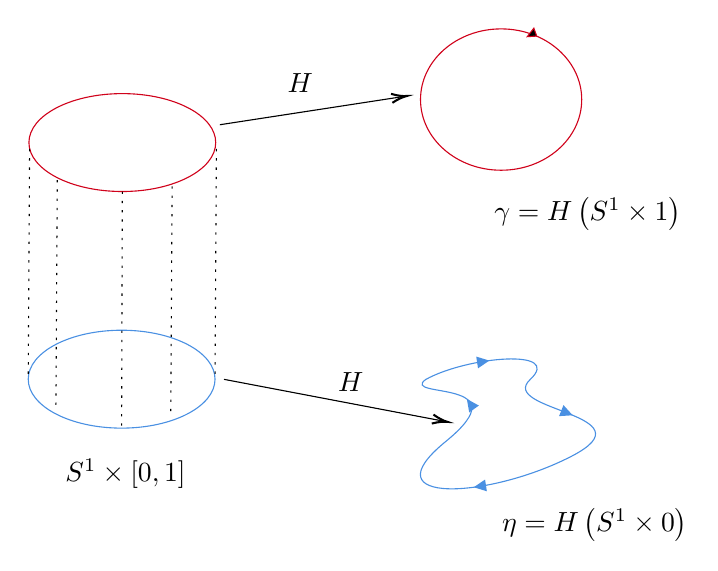
\begin{tikzpicture}[x=0.5pt,y=0.5pt,yscale=-1,xscale=1]
%uncomment if require: \path (0,414); %set diagram left start at 0, and has height of 414

%Shape: Ellipse [id:dp8580791830403575] 
\draw  [color={rgb, 255:red, 208; green, 2; blue, 27 }  ,draw opacity=1 ] (344.5,83.8) .. controls (344.5,55.59) and (370.58,32.73) .. (402.75,32.73) .. controls (434.92,32.73) and (461,55.59) .. (461,83.8) .. controls (461,112) and (434.92,134.87) .. (402.75,134.87) .. controls (370.58,134.87) and (344.5,112) .. (344.5,83.8) -- cycle ;
%Shape: Triangle [id:dp1741505392127638] 
\draw  [color={rgb, 255:red, 208; green, 2; blue, 27 }  ,draw opacity=1 ][fill={rgb, 255:red, 0; green, 0; blue, 0 }  ,fill opacity=1 ] (428.46,37.93) -- (421.68,38.35) -- (426.41,32.25) -- cycle ;

%Curve Lines [id:da2246700601326841] 
\draw [color={rgb, 255:red, 74; green, 144; blue, 226 }  ,draw opacity=1 ]   (348.25,286.09) .. controls (378.46,269.4) and (447.94,263.42) .. (423.78,286.09) .. controls (399.61,308.76) and (512.89,310.99) .. (453.61,341.59) .. controls (394.32,372.19) and (305.96,377.19) .. (362.6,331.02) .. controls (419.25,284.84) and (329.37,300) .. (348.25,286.09) -- cycle ;
\draw [shift={(394.24,272.44)}, rotate = 171.27] [fill={rgb, 255:red, 74; green, 144; blue, 226 }  ,fill opacity=1 ][line width=0.08]  [draw opacity=0] (8.93,-4.29) -- (0,0) -- (8.93,4.29) -- cycle    ;
\draw [shift={(454.51,311.96)}, rotate = 201.95] [fill={rgb, 255:red, 74; green, 144; blue, 226 }  ,fill opacity=1 ][line width=0.08]  [draw opacity=0] (8.93,-4.29) -- (0,0) -- (8.93,4.29) -- cycle    ;
\draw [shift={(382.98,363.98)}, rotate = 351.41] [fill={rgb, 255:red, 74; green, 144; blue, 226 }  ,fill opacity=1 ][line width=0.08]  [draw opacity=0] (8.93,-4.29) -- (0,0) -- (8.93,4.29) -- cycle    ;
\draw [shift={(377.98,300.18)}, rotate = 54.37] [fill={rgb, 255:red, 74; green, 144; blue, 226 }  ,fill opacity=1 ][line width=0.08]  [draw opacity=0] (8.93,-4.29) -- (0,0) -- (8.93,4.29) -- cycle    ;

%Shape: Ellipse [id:dp5051354795111995] 
\draw  [color={rgb, 255:red, 208; green, 2; blue, 27 }  ,draw opacity=1 ] (61.5,114.88) .. controls (61.5,95.34) and (91.72,79.5) .. (129,79.5) .. controls (166.28,79.5) and (196.5,95.34) .. (196.5,114.88) .. controls (196.5,134.41) and (166.28,150.25) .. (129,150.25) .. controls (91.72,150.25) and (61.5,134.41) .. (61.5,114.88) -- cycle ;
%Shape: Ellipse [id:dp028752110313813417] 
\draw  [color={rgb, 255:red, 74; green, 144; blue, 226 }  ,draw opacity=1 ] (61,285.88) .. controls (61,266.34) and (91.22,250.5) .. (128.5,250.5) .. controls (165.78,250.5) and (196,266.34) .. (196,285.88) .. controls (196,305.41) and (165.78,321.25) .. (128.5,321.25) .. controls (91.22,321.25) and (61,305.41) .. (61,285.88) -- cycle ;
%Straight Lines [id:da6715965743533834] 
\draw  [dash pattern={on 0.84pt off 2.51pt}]  (62,119.5) -- (61,285.88) ;
%Straight Lines [id:da24973361821393547] 
\draw  [dash pattern={on 0.84pt off 2.51pt}]  (82,142) -- (81,308.38) ;
%Straight Lines [id:da664998350332383] 
\draw  [dash pattern={on 0.84pt off 2.51pt}]  (129,150.25) -- (128.5,321.25) ;
%Straight Lines [id:da0662385964287534] 
\draw  [dash pattern={on 0.84pt off 2.51pt}]  (165,146.5) -- (164,312.88) ;
%Straight Lines [id:da3891917682172963] 
\draw  [dash pattern={on 0.84pt off 2.51pt}]  (197,119.5) -- (196,285.88) ;
%Straight Lines [id:da7252691499439365] 
\draw    (199.5,102) -- (332.52,81.55) ;
\draw [shift={(334.5,81.25)}, rotate = 171.26] [color={rgb, 255:red, 0; green, 0; blue, 0 }  ][line width=0.75]    (10.93,-3.29) .. controls (6.95,-1.4) and (3.31,-0.3) .. (0,0) .. controls (3.31,0.3) and (6.95,1.4) .. (10.93,3.29)   ;
%Straight Lines [id:da7874706184444381] 
\draw    (202.5,286) -- (362.04,316.38) ;
\draw [shift={(364,316.75)}, rotate = 190.78] [color={rgb, 255:red, 0; green, 0; blue, 0 }  ][line width=0.75]    (10.93,-3.29) .. controls (6.95,-1.4) and (3.31,-0.3) .. (0,0) .. controls (3.31,0.3) and (6.95,1.4) .. (10.93,3.29)   ;

% Text Node
\draw (401.54,377.52) node [anchor=north west][inner sep=0.75pt]    {$\eta =H\left( S^{1} \times 0\right)$};
% Text Node
\draw (396.02,152.8) node [anchor=north west][inner sep=0.75pt]    {$\gamma =H\left( S^{1} \times 1\right)$};
% Text Node
\draw (246.5,63.4) node [anchor=north west][inner sep=0.75pt]    {$H$};
% Text Node
\draw (283,278.9) node [anchor=north west][inner sep=0.75pt]    {$H$};
% Text Node
\draw (86,341.9) node [anchor=north west][inner sep=0.75pt]    {$S^{1} \times [ 0,1]$};


\end{tikzpicture}

    \caption{Representation of $H$}
    \label{fig:my_label}
\end{figure}
\textbf{Winding number: }It is the total number of loops we make when we complete traversing closed curve. Alternatively, imagine holding out a compass needle. Then the total number of complete turns the needle makes will be the winding number.
\begin{figure}[!htb]
    \centering
    

\tikzset{every picture/.style={line width=0.75pt}} %set default line width to 0.75pt        

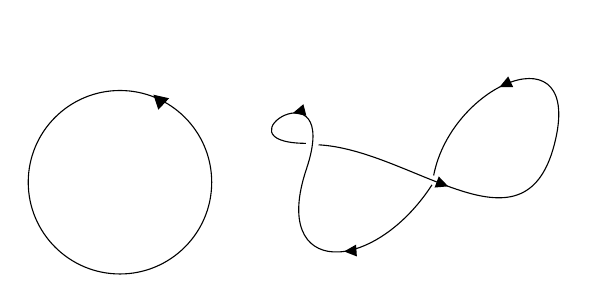
\begin{tikzpicture}[x=0.5pt,y=0.5pt,yscale=-1,xscale=1]
%uncomment if require: \path (0,300); %set diagram left start at 0, and has height of 300

%Shape: Circle [id:dp9595274264781469] 
\draw   (40,105.9) .. controls (40,69.28) and (69.68,39.6) .. (106.3,39.6) .. controls (142.92,39.6) and (172.6,69.28) .. (172.6,105.9) .. controls (172.6,142.52) and (142.92,172.2) .. (106.3,172.2) .. controls (69.68,172.2) and (40,142.52) .. (40,105.9) -- cycle ;
%Curve Lines [id:da6184433689903426] 
\draw    (240.6,77.8) .. controls (173,77.4) and (267.4,17.8) .. (240.99,96.55) .. controls (214.59,175.31) and (289.21,173.29) .. (331.8,107.8) ;
\draw [shift={(231.29,55.9)}, rotate = 345.54] [fill={rgb, 255:red, 0; green, 0; blue, 0 }  ][line width=0.08]  [draw opacity=0] (8.93,-4.29) -- (0,0) -- (8.93,4.29) -- cycle    ;
\draw [shift={(268.31,155.91)}, rotate = 355.98] [fill={rgb, 255:red, 0; green, 0; blue, 0 }  ][line width=0.08]  [draw opacity=0] (8.93,-4.29) -- (0,0) -- (8.93,4.29) -- cycle    ;
%Curve Lines [id:da37718589291443505] 
\draw    (249.79,78.86) .. controls (317.6,82.53) and (398.11,163.13) .. (420.15,78.86) .. controls (442.2,-5.4) and (345.95,33.94) .. (333,101) ;
\draw [shift={(343.53,108.87)}, rotate = 200.62] [fill={rgb, 255:red, 0; green, 0; blue, 0 }  ][line width=0.08]  [draw opacity=0] (8.93,-4.29) -- (0,0) -- (8.93,4.29) -- cycle    ;
\draw [shift={(380.59,37.11)}, rotate = 334.94] [fill={rgb, 255:red, 0; green, 0; blue, 0 }  ][line width=0.08]  [draw opacity=0] (8.93,-4.29) -- (0,0) -- (8.93,4.29) -- cycle    ;
%Shape: Triangle [id:dp8787590147736832] 
\draw  [fill={rgb, 255:red, 0; green, 0; blue, 0 }  ,fill opacity=1 ] (134.18,52.72) -- (131.09,43.21) -- (141.04,45.45) -- cycle ;




\end{tikzpicture}

    \caption{Winding number 1}
    \label{fig:my_label}
\end{figure}

\begin{figure}[!htb]
    \centering
    

\tikzset{every picture/.style={line width=0.75pt}} %set default line width to 0.75pt        

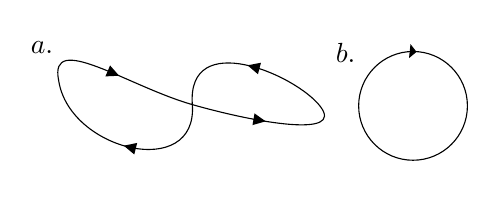
\begin{tikzpicture}[x=0.5pt,y=0.5pt,yscale=-1,xscale=1]
%uncomment if require: \path (0,300); %set diagram left start at 0, and has height of 300

%Curve Lines [id:da2718429255912467] 
\draw    (43.6,41.2) .. controls (36.2,5) and (93.8,45.4) .. (140.2,58.6) .. controls (186.6,71.8) and (250.6,83) .. (232.6,59.8) .. controls (214.6,36.6) and (136.2,3.4) .. (140.2,58.6) .. controls (144.2,113.8) and (51.4,92.2) .. (43.6,41.2) -- cycle ;
\draw [shift={(87.29,37.75)}, rotate = 203.05] [fill={rgb, 255:red, 0; green, 0; blue, 0 }  ][line width=0.08]  [draw opacity=0] (8.93,-4.29) -- (0,0) -- (8.93,4.29) -- cycle    ;
\draw [shift={(193.2,70.68)}, rotate = 189.74] [fill={rgb, 255:red, 0; green, 0; blue, 0 }  ][line width=0.08]  [draw opacity=0] (8.93,-4.29) -- (0,0) -- (8.93,4.29) -- cycle    ;
\draw [shift={(180.08,30.21)}, rotate = 14.73] [fill={rgb, 255:red, 0; green, 0; blue, 0 }  ][line width=0.08]  [draw opacity=0] (8.93,-4.29) -- (0,0) -- (8.93,4.29) -- cycle    ;
\draw [shift={(90.63,88.3)}, rotate = 14.01] [fill={rgb, 255:red, 0; green, 0; blue, 0 }  ][line width=0.08]  [draw opacity=0] (8.93,-4.29) -- (0,0) -- (8.93,4.29) -- cycle    ;
%Shape: Circle [id:dp8907209896109666] 
\draw   (260.4,59.5) .. controls (260.4,37.8) and (278,20.2) .. (299.7,20.2) .. controls (321.4,20.2) and (339,37.8) .. (339,59.5) .. controls (339,81.2) and (321.4,98.8) .. (299.7,98.8) .. controls (278,98.8) and (260.4,81.2) .. (260.4,59.5) -- cycle ;
%Shape: Triangle [id:dp6641882002067809] 
\draw  [fill={rgb, 255:red, 0; green, 0; blue, 0 }  ,fill opacity=1 ] (301.69,20.41) -- (297.29,24.07) -- (298.14,15.91) -- cycle ;

% Text Node
\draw (21.6,11.2) node [anchor=north west][inner sep=0.75pt]    {$a.$};
% Text Node
\draw (242,12.6) node [anchor=north west][inner sep=0.75pt]    {$b.$};


\end{tikzpicture}

    \caption{a. Winding number 0 b. Winding number -1}
    \label{fig:my_label}
\end{figure}

But what if we consider curves in $S^2$? Then the theorem changes as follows:

\begin{theorem}[Hirsch-Smale Theory, $2^{nd}$ part]
Any two immersed loop in $S^2$ are isotopic if and only if the winding numbers match modulo 2.
\end{theorem}
\begin{figure*}[!htb]
    \centering
    

% Gradient Info
  
\tikzset {_o50ed9ycy/.code = {\pgfsetadditionalshadetransform{ \pgftransformshift{\pgfpoint{0 bp } { 0 bp }  }  \pgftransformscale{1 }  }}}
\pgfdeclareradialshading{_gk5204urd}{\pgfpoint{0bp}{0bp}}{rgb(0bp)=(1,1,1);
rgb(0bp)=(1,1,1);
rgb(25bp)=(0.29,0.56,0.89);
rgb(400bp)=(0.29,0.56,0.89)}

% Gradient Info
  
\tikzset {_2m37d3yfb/.code = {\pgfsetadditionalshadetransform{ \pgftransformshift{\pgfpoint{0 bp } { 0 bp }  }  \pgftransformscale{1 }  }}}
\pgfdeclareradialshading{_6smwnwe06}{\pgfpoint{0bp}{0bp}}{rgb(0bp)=(1,1,1);
rgb(0bp)=(1,1,1);
rgb(25bp)=(0.29,0.56,0.89);
rgb(400bp)=(0.29,0.56,0.89)}

% Gradient Info
  
\tikzset {_b6wkzg2sw/.code = {\pgfsetadditionalshadetransform{ \pgftransformshift{\pgfpoint{0 bp } { 0 bp }  }  \pgftransformscale{1 }  }}}
\pgfdeclareradialshading{_s15twwqz4}{\pgfpoint{0bp}{0bp}}{rgb(0bp)=(1,1,1);
rgb(0bp)=(1,1,1);
rgb(25bp)=(0.29,0.56,0.89);
rgb(400bp)=(0.29,0.56,0.89)}
\tikzset{every picture/.style={line width=0.75pt}} %set default line width to 0.75pt        

\begin{tikzpicture}[x=0.75pt,y=0.75pt,yscale=-1,xscale=1]
%uncomment if require: \path (0,300); %set diagram left start at 0, and has height of 300

%Shape: Circle [id:dp4428149399613551] 
\path  [shading=_gk5204urd,_o50ed9ycy] (40.8,131.5) .. controls (40.8,86.82) and (77.02,50.6) .. (121.7,50.6) .. controls (166.38,50.6) and (202.6,86.82) .. (202.6,131.5) .. controls (202.6,176.18) and (166.38,212.4) .. (121.7,212.4) .. controls (77.02,212.4) and (40.8,176.18) .. (40.8,131.5) -- cycle ; % for fading 
 \draw  [color={rgb, 255:red, 74; green, 144; blue, 226 }  ,draw opacity=1 ] (40.8,131.5) .. controls (40.8,86.82) and (77.02,50.6) .. (121.7,50.6) .. controls (166.38,50.6) and (202.6,86.82) .. (202.6,131.5) .. controls (202.6,176.18) and (166.38,212.4) .. (121.7,212.4) .. controls (77.02,212.4) and (40.8,176.18) .. (40.8,131.5) -- cycle ; % for border 

%Shape: Circle [id:dp10055389125205716] 
\draw  [color={rgb, 255:red, 208; green, 2; blue, 27 }  ,draw opacity=1 ] (81.6,131.5) .. controls (81.6,109.35) and (99.55,91.4) .. (121.7,91.4) .. controls (143.85,91.4) and (161.8,109.35) .. (161.8,131.5) .. controls (161.8,153.65) and (143.85,171.6) .. (121.7,171.6) .. controls (99.55,171.6) and (81.6,153.65) .. (81.6,131.5) -- cycle ;
%Shape: Triangle [id:dp3509374145983808] 
\draw  [fill={rgb, 255:red, 0; green, 0; blue, 0 }  ,fill opacity=1 ] (125,91.5) -- (118.29,95) -- (118.51,87.61) -- cycle ;
%Straight Lines [id:da5671120603581383] 
\draw    (210.8,119.6) -- (274.2,120.57) ;
\draw [shift={(276.2,120.6)}, rotate = 180.88] [color={rgb, 255:red, 0; green, 0; blue, 0 }  ][line width=0.75]    (10.93,-3.29) .. controls (6.95,-1.4) and (3.31,-0.3) .. (0,0) .. controls (3.31,0.3) and (6.95,1.4) .. (10.93,3.29)   ;
%Curve Lines [id:da8668609867265892] 
\draw  [dash pattern={on 4.5pt off 4.5pt}]  (156.8,100.4) .. controls (156.21,59.25) and (175.97,39.21) .. (196.98,53.44) ;
\draw [shift={(198.6,54.6)}, rotate = 217.21] [color={rgb, 255:red, 0; green, 0; blue, 0 }  ][line width=0.75]    (10.93,-3.29) .. controls (6.95,-1.4) and (3.31,-0.3) .. (0,0) .. controls (3.31,0.3) and (6.95,1.4) .. (10.93,3.29)   ;
%Curve Lines [id:da49265357313711355] 
\draw  [dash pattern={on 4.5pt off 4.5pt}]  (80.8,100.4) .. controls (80.21,58.83) and (73.99,27.55) .. (51.25,57.2) ;
\draw [shift={(50.2,58.6)}, rotate = 306.41] [color={rgb, 255:red, 0; green, 0; blue, 0 }  ][line width=0.75]    (10.93,-3.29) .. controls (6.95,-1.4) and (3.31,-0.3) .. (0,0) .. controls (3.31,0.3) and (6.95,1.4) .. (10.93,3.29)   ;
%Curve Lines [id:da05561541607024678] 
\draw  [dash pattern={on 4.5pt off 4.5pt}]  (160,168.8) .. controls (159.8,219.56) and (238.94,217.51) .. (222.9,191.43) ;
\draw [shift={(221.8,189.8)}, rotate = 53.53] [color={rgb, 255:red, 0; green, 0; blue, 0 }  ][line width=0.75]    (10.93,-3.29) .. controls (6.95,-1.4) and (3.31,-0.3) .. (0,0) .. controls (3.31,0.3) and (6.95,1.4) .. (10.93,3.29)   ;
%Curve Lines [id:da23945267738357534] 
\draw  [dash pattern={on 4.5pt off 4.5pt}]  (88.4,169.6) .. controls (88.2,220.88) and (36.84,239.04) .. (41.64,193.21) ;
\draw [shift={(41.8,191.8)}, rotate = 97.18] [color={rgb, 255:red, 0; green, 0; blue, 0 }  ][line width=0.75]    (10.93,-3.29) .. controls (6.95,-1.4) and (3.31,-0.3) .. (0,0) .. controls (3.31,0.3) and (6.95,1.4) .. (10.93,3.29)   ;
%Shape: Circle [id:dp8287841133971156] 
\path  [shading=_6smwnwe06,_2m37d3yfb] (286.8,122.7) .. controls (286.8,78.02) and (323.02,41.8) .. (367.7,41.8) .. controls (412.38,41.8) and (448.6,78.02) .. (448.6,122.7) .. controls (448.6,167.38) and (412.38,203.6) .. (367.7,203.6) .. controls (323.02,203.6) and (286.8,167.38) .. (286.8,122.7) -- cycle ; % for fading 
 \draw  [color={rgb, 255:red, 74; green, 144; blue, 226 }  ,draw opacity=1 ] (286.8,122.7) .. controls (286.8,78.02) and (323.02,41.8) .. (367.7,41.8) .. controls (412.38,41.8) and (448.6,78.02) .. (448.6,122.7) .. controls (448.6,167.38) and (412.38,203.6) .. (367.7,203.6) .. controls (323.02,203.6) and (286.8,167.38) .. (286.8,122.7) -- cycle ; % for border 

%Shape: Circle [id:dp3582440477404123] 
\draw  [color={rgb, 255:red, 208; green, 2; blue, 27 }  ,draw opacity=1 ][dash pattern={on 4.5pt off 4.5pt}] (327.6,122.7) .. controls (327.6,100.55) and (345.55,82.6) .. (367.7,82.6) .. controls (389.85,82.6) and (407.8,100.55) .. (407.8,122.7) .. controls (407.8,144.85) and (389.85,162.8) .. (367.7,162.8) .. controls (345.55,162.8) and (327.6,144.85) .. (327.6,122.7) -- cycle ;
%Shape: Triangle [id:dp57592370617849] 
\draw  [fill={rgb, 255:red, 0; green, 0; blue, 0 }  ,fill opacity=1 ] (354.35,85.34) -- (349.67,91.28) -- (346.84,84.44) -- cycle ;
%Straight Lines [id:da6906001583873703] 
\draw    (368.2,19.8) -- (367.2,225.6) ;
%Curve Lines [id:da47646965878996683] 
\draw    (350.2,31) .. controls (300.81,50.21) and (434.28,50.21) .. (394.83,31) ;
\draw [shift={(392.2,29.8)}, rotate = 23.2] [fill={rgb, 255:red, 0; green, 0; blue, 0 }  ][line width=0.08]  [draw opacity=0] (8.93,-4.29) -- (0,0) -- (8.93,4.29) -- cycle    ;
%Shape: Circle [id:dp6404134705913701] 
\path  [shading=_s15twwqz4,_b6wkzg2sw] (522.8,119.1) .. controls (522.8,74.42) and (559.02,38.2) .. (603.7,38.2) .. controls (648.38,38.2) and (684.6,74.42) .. (684.6,119.1) .. controls (684.6,163.78) and (648.38,200) .. (603.7,200) .. controls (559.02,200) and (522.8,163.78) .. (522.8,119.1) -- cycle ; % for fading 
 \draw  [color={rgb, 255:red, 74; green, 144; blue, 226 }  ,draw opacity=1 ] (522.8,119.1) .. controls (522.8,74.42) and (559.02,38.2) .. (603.7,38.2) .. controls (648.38,38.2) and (684.6,74.42) .. (684.6,119.1) .. controls (684.6,163.78) and (648.38,200) .. (603.7,200) .. controls (559.02,200) and (522.8,163.78) .. (522.8,119.1) -- cycle ; % for border 

%Shape: Circle [id:dp020289716418068426] 
\draw  [color={rgb, 255:red, 208; green, 2; blue, 27 }  ,draw opacity=1 ] (563.6,119.1) .. controls (563.6,96.95) and (581.55,79) .. (603.7,79) .. controls (625.85,79) and (643.8,96.95) .. (643.8,119.1) .. controls (643.8,141.25) and (625.85,159.2) .. (603.7,159.2) .. controls (581.55,159.2) and (563.6,141.25) .. (563.6,119.1) -- cycle ;
%Shape: Triangle [id:dp8243051535367023] 
\draw  [fill={rgb, 255:red, 0; green, 0; blue, 0 }  ,fill opacity=1 ] (600.4,79.05) -- (606.94,75.25) -- (607.05,82.65) -- cycle ;
%Straight Lines [id:da5989560347824799] 
\draw    (452.4,119.2) -- (515.8,120.17) ;
\draw [shift={(517.8,120.2)}, rotate = 180.88] [color={rgb, 255:red, 0; green, 0; blue, 0 }  ][line width=0.75]    (10.93,-3.29) .. controls (6.95,-1.4) and (3.31,-0.3) .. (0,0) .. controls (3.31,0.3) and (6.95,1.4) .. (10.93,3.29)   ;




\end{tikzpicture}

    \caption{Example of part two of theorem. The winding number changes from -1 to +1. The dotted lines represent the curve on the rear side of the sphere.}
    \label{fig:my_label}
\end{figure*}

\chapter{Curves}
\section{Introduction}
We shall first consider some probable definitions of curves and see why they are wrong.
\begin{enumerate}
    \item \textbf{A curve is a set with empty interior}. This on the first glance looks pretty good: after all our by our geometric intuition, a curve has nothing inside it. But while it does take into account all things we intuitively understand as curve, there are things included in this which are not very curve like. For example, consider:
    $$f(x,y)=\begin{cases}1\quad&x\in\mathbb Q\times\mathbb Q\\ 0\quad&x\notin\mathbb Q\times\mathbb Q\end{cases}$$
    As $\mathbb Q$ is dense in $\mathbb R$, $S=\{(x,y)|f(x,y)=0\}$ has a empty interior. But it's obvious that $S$ which has some weird appearance is definitely not a curve.
  \item\textbf{A curve is the graph of a function.} Therefore, every curve can be represented as $(x,f(x))$ or $(x,f_1(x),f_2(x))$. This definition suffers from the opposite problem of the previous definition. Note, structures like a vertical line($y=k$) or a parabola($x=y^2$) can not be graphs of functions because they fail the vertical line test and are yet curves.
  \begin{figure}[H]
      \centering
      

\tikzset{every picture/.style={line width=0.75pt}} %set default line width to 0.75pt        

\begin{tikzpicture}[x=0.75pt,y=0.75pt,yscale=-1,xscale=1]
%uncomment if require: \path (0,300); %set diagram left start at 0, and has height of 300

%Curve Lines [id:da21071482613616144] 
\draw    (32.33,14.17) .. controls (78,15.5) and (-23.67,80.83) .. (39,55.83) .. controls (101.67,30.83) and (-2.67,105.5) .. (38,113.17) ;
%Shape: Arc [id:dp004048976867261689] 
\draw  [draw opacity=0] (155.45,96.51) .. controls (151.7,96.94) and (147.81,97.17) .. (143.83,97.17) .. controls (111.89,97.17) and (86,82.58) .. (86,64.58) .. controls (86,46.59) and (111.89,32) .. (143.83,32) .. controls (162.24,32) and (178.63,36.84) .. (189.23,44.39) -- (143.83,64.58) -- cycle ; \draw   (155.45,96.51) .. controls (151.7,96.94) and (147.81,97.17) .. (143.83,97.17) .. controls (111.89,97.17) and (86,82.58) .. (86,64.58) .. controls (86,46.59) and (111.89,32) .. (143.83,32) .. controls (162.24,32) and (178.63,36.84) .. (189.23,44.39) ;
%Straight Lines [id:da4986095954483222] 
\draw  [dash pattern={on 0.84pt off 2.51pt}]  (39,7.33) -- (38.33,118.17) ;
%Straight Lines [id:da8847804148280588] 
\draw  [dash pattern={on 0.84pt off 2.51pt}]  (120,8.33) -- (120,117.5) ;




\end{tikzpicture}

      \caption{Two curves which are not graphs of a function}
      \label{fig:my_label}
  \end{figure}
  \item\textbf{A curve is the set of points where a function vanishes.} We might think this works: after all, we can now circumnavigate around our previous problem by making an suitable function like $f(x,y):=y-k$ or $f(x,y):=x-y^2$. But this again makes things which are intuitively not a curve, a curve.
  \begin{figure}[H]
      \centering
      

\tikzset{every picture/.style={line width=0.75pt}} %set default line width to 0.75pt        

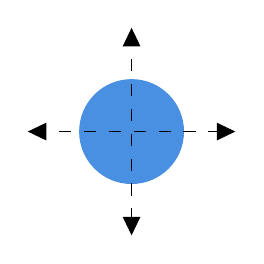
\begin{tikzpicture}[x=0.75pt,y=0.75pt,yscale=-1,xscale=1]
%uncomment if require: \path (0,300); %set diagram left start at 0, and has height of 300

%Shape: Circle [id:dp36858899353733066] 
\draw  [color={rgb, 255:red, 74; green, 144; blue, 226 }  ,draw opacity=1 ][fill={rgb, 255:red, 74; green, 144; blue, 226 }  ,fill opacity=1 ] (75,100) .. controls (75,86.19) and (86.19,75) .. (100,75) .. controls (113.81,75) and (125,86.19) .. (125,100) .. controls (125,113.81) and (113.81,125) .. (100,125) .. controls (86.19,125) and (75,113.81) .. (75,100) -- cycle ;
%Straight Lines [id:da8206727916415146] 
\draw  [dash pattern={on 4.5pt off 4.5pt}]  (100,53) -- (100,147) ;
\draw [shift={(100,150)}, rotate = 270] [fill={rgb, 255:red, 0; green, 0; blue, 0 }  ][line width=0.08]  [draw opacity=0] (8.93,-4.29) -- (0,0) -- (8.93,4.29) -- cycle    ;
\draw [shift={(100,50)}, rotate = 90] [fill={rgb, 255:red, 0; green, 0; blue, 0 }  ][line width=0.08]  [draw opacity=0] (8.93,-4.29) -- (0,0) -- (8.93,4.29) -- cycle    ;
%Straight Lines [id:da5344450574564665] 
\draw  [dash pattern={on 4.5pt off 4.5pt}]  (53,100) -- (147,100) ;
\draw [shift={(150,100)}, rotate = 180] [fill={rgb, 255:red, 0; green, 0; blue, 0 }  ][line width=0.08]  [draw opacity=0] (8.93,-4.29) -- (0,0) -- (8.93,4.29) -- cycle    ;
\draw [shift={(50,100)}, rotate = 0] [fill={rgb, 255:red, 0; green, 0; blue, 0 }  ][line width=0.08]  [draw opacity=0] (8.93,-4.29) -- (0,0) -- (8.93,4.29) -- cycle    ;




\end{tikzpicture}

      \caption{Set $f(x,y)=\max\{x^2+y^2-1,0\}$. The resulting figure, clearly, doesn't form something we would like to recognise as a curve}
      \label{fig:my_label}
  \end{figure}
\end{enumerate}

\section{Whitney's Teorem}
\begin{theorem}[Whitney's Theorem]
Let $\Omega\in\mathbb R^n$ be any open subset. Given a closed $C\subseteq \Omega$, there exists a smooth function $f:\Omega\to\mathbb R$ such that $C=f^{-1}(0)$
\end{theorem}
\begin{proof}
\textbf{Step 1(Covering): }Note, $V=\Omega\setminus C$ is open in $\Omega$(and in fact, it is also open in $\mathbb R^n$). We want to cover this by a collection of open balls. We do this by taking every $q_n(\in\mathbb Q\times\mathbb Q\hdots)$ and an appropriate radius for each $q_n$. Therefore:
$$V=\bigcup_{k} B(\overrightarrow{p_k},r_k)\quad[\overrightarrow{p_k}\in\mathbb Q^n\cap V,r_k\in\mathbb Q]$$
Note, this is a covering of $V$ because $Q$ is dense in $\mathbb R$.\\
\textbf{Step 2(Choosing Bump Functions): }Choose $f_k:\mathbb R^n\to \mathbb R$(those are smooth functions) such that $$f_k^{-1}(0)=\mathbb R^n\setminus B(\overrightarrow{p_k},r_k)$$
$$f_k^{-1}(1)=\overline{ B(\overrightarrow{p_k},r_k/2)}$$
This has been done as solution to problem 2 in exercise 1. Essentially, this looks like a smooth pudding(I feel sand heap is a better example) with a flat top. Moreover, all derivative of $f_k$ vanishes on $\mathbb R^n\setminus \overline{B(\overrightarrow{p_k},r_k)}$\\
\textbf{Step 3(Combining those functions): }We want to combine(by adding) those bump functions appropriately with weights such that the partial sums converge uniformly and their derivatives converge uniformly too. Note, for every point outside the closed set, it is present in some open ball with the bump. Therefore, if we assign a positive weight to every bump function, then , if the sum converges, $f^{-1}(0)=C$ as all the other points lie in some bump. We define 
$$c_k=\max_{|\alpha|\leq k,\overrightarrow{y}\in \overline{B(\overrightarrow{p_k},r_k)}}\left|\frac{\partial^\alpha}{\partial x^m}f_k(\overrightarrow{y})\right|$$
\textit{Note on notation:} $\alpha$ is a \textit{multi-index} and each $x^m$ is differentiation w.r.t a particular index $\alpha$ times. For example, if $\alpha=(1,0,2)$, it would mean $\frac{\partial^3}{\partial x_1\partial x_3^2}f_k(x)$. As $f_k$ is assumed to be smooth, order of derivatives don't matter. In particular, for $\alpha=1$, the max will be calculated between $f(\overline{y}),\frac{\partial}{\partial x_1}(\overline{y}),\frac{\partial}{\partial x_2}(\overline{y}),\frac{\partial}{\partial x_3}(\overline{y})$ on the whole set.\\
Now as $f$ and it's derivative are continuous and we are considering the maximum on a compact set, $c_k$ is well defined and exists. Those $c_k$ will become our weights. We define $f$ as
$$f=\sum_{k=0}^\infty \frac{f_k}{2^kc_k}$$

\textbf{Step 4(Analytical verification): }\\
Check $f^{-1}(0)=C$. If $\overrightarrow{p}\ne C$ then $\overrightarrow{p}\in V$, whence $\overrightarrow{p}\in B(\overrightarrow{p_k},r_k)$, then $f(p)>\frac{f_k(p)}{2^kc_k}>0$. If  $\overrightarrow{p}\in C$, then $p\notin B(\overrightarrow{p_k},r_k)$ for any $k$ so $f(p)=0$. Now we show $f$ is $C^0$, by showing convergence of the sequence of $f$. Given $\epsilon>0$ choose $N$ such that $\frac{1}{2^N}<\epsilon$. Compare $S_m(f)$ and $S_n(f)$ with $m>n\geq N$. $S_n(f)$ is the partial sum $\sum_{k=1}^n \frac{f_k}{2^kc_k}$. Note:
$$\sup_{x\in \mathbb R^n}|f_m(x)-f_n(x)|=\sum_{i=m}^n \frac{f_k}{2^kc_k}\leq \sum_{i=m}^n \frac{1}{2^k}\leq \sum_{i=m}^\infty \frac{1}{2^k}\leq \frac{1}{2^{m}}$$
The thing to note is we have $\frac{f_k}{c_k}<1$ due to how $c_k$ is defined. For higher derivatives it still holds(again, due to how $c_k$ is defined) albeit with slight modifications. The $1/2^k$ is present to ensure convergence.\\\\
\textit{Note: This theorem is not very important in this course but the proof shows a classic old trick: finding covers, attaching weights and then performing analysis to get the desired result.}
\end{proof}




\section{Parameterized Curve}
\begin{definition}[Parameterized Curve]
A paameterized smooth curve is a smooth function $\gamma:(a,b)\to\mathbb R^n$ where $-\infty\leq a\leq b\leq \infty$.(we include $\pm\infty$ as the function may map the whole of $\mathbb R$ to $\mathbb R^n$).
\end{definition}
Generally, we use lower Greek letters (like $\eta,\varphi,$ etc.) to denote curves.
\subsection{Reparameterization of curve}
\begin{definition}[Reparameterization of a curve]
Let $\varphi(\alpha',\beta')\to(\alpha,\beta)$ be a homeomorphism.
If $\gamma$ is a parameterised curve as defined above, then $\eta:(\alpha',\beta')\to\mathbb R^n,\eta=\gamma\circ\varphi$ is called the reparameterization of $\gamma$.
\end{definition}

If $\varphi$ is a diffeomorphism and $\gamma$ is smooth then $\eta$ is smooth. (see appendix, section 4). In particular, if $\gamma$ is $C^k$ then $\eta$ is $C^k$ if $\varphi$ is diffeomorphism. 
$$\eta'(t)=\underbrace{\gamma'(\varphi(t))}_{=Vector}\underbrace{\varphi'(t)}_{=Scalar}$$
If $\varphi$ is $C^0$ then $\varphi$ is monotonic. This is ascertained by the intermediate value theorem. If $\varphi$ is atleast $C^1$ then we can further confirm $\varphi\ne 0$. Let $\psi$ be the inverse of $\varphi$. Then:
$$\psi\circ \varphi(x)=x\Rightarrow \psi'(\varphi(x))\varphi'(x)=1$$
Therefore, $\varphi(x)\ne0$ and $\varphi$ is strictly increasing or strictly decreasing. If $\varphi(\alpha')=\alpha',\varphi(\beta')=\beta$ then $\eta$ is orientation preserving and if  $\varphi(\alpha')=\beta',\varphi(\beta)=\alpha'$ then $\eta$ is orientation reversing. 

\subsection{Arc length parameter}
\begin{definition}[Arc-Length]
The arc length of a differentiable curve $\gamma(\alpha,\beta)\to\mathbb R^n$ starting at $t_0$ is defined as:
$$S(t)=\int_{t_o}^t||\gamma'(u)||du$$
\end{definition}
This formula is quite intutive. We can consider the curve to be path of a particle, $\gamma(u)$ to be the position at time $u$. Then $\gamma'(u)$ gives the velocity at $u$ and taking it's magnitude gives the speed. Integrating speed at various points gives the distance covered, or in this case, length of the arc traversed.\\
As $\gamma'$ is atleast $C^0$ and the interval is closed and bounded, the integral is well defined and finite. Moreover:
$$\frac{d}{dt}S(t)=||\gamma'(t)||$$
\begin{definition}[Regular Curve]
A curve $\gamma$ is called regular if $\gamma'\ne0$
\end{definition}
\textbf{Example: }A curve with unit speed(i.e $||\gamma'(u)||=1$ everywhere).
\begin{lemma}
\begin{enumerate}
    \item Let $\gamma(\alpha,\beta)\to\mathbb R^n$ be a regular smooth curve. Then the arc length parameter $S$ is smooth function of $t$.
    \item The arc length parameter is a diffeomorphism onto it's image.
    \item Let $\varphi$ denote tha map: $S^{-1}(\tilde\alpha,\tilde\beta)\to(\alpha,\beta)$. Then $\gamma\circ\varphi$ is a unit speed curve reaparameterization.
    \item Any other unit speed reparameterization is a shift or reflection of the above.
\end{enumerate}
\end{lemma}
\begin{proof}
\begin{enumerate}
    \item As $\gamma'$ is smooth and $<,>$ is smooth, we know $<\gamma'(t),\gamma'(t)>$ is smooth. Therefore:
    $\frac{ds}{dt}=||\gamma'(t)||=\sqrt{<\gamma'(t),\gamma'(t)>}$ is a composition of smooth function and is smooth.(\textit{Note:} the distance function is not smooth around zero, but this poses no problem as the curve is regular).
    \item Inverse of smooth function is smooth and as $||\gamma'(t)||>0$, $S$ is monotonic. So $S$ is smooth,invertible and has a smooth inverse.
    \item Note that:
    $$S\circ \varphi (t)=t\Rightarrow S'(\varphi(t))\varphi'(t)=1$$
    Therefore:
    $$||(\gamma\circ\varphi)'(t)||=|\varphi'(t)|\times ||\gamma'(\varphi(t)) ||=|\varphi'(t)|S'(\varphi(t))=1$$
    The key step involves noting $||\gamma'(\varphi(t))||=\frac{d}{dt}S(\varphi(t))$
    \item This is proved in homework 3
\end{enumerate}
\end{proof}

\section{Bending of a curve: Curvature}






























\onecolumn
\chapter{Homework Solutions}
\section{Homework 1}
Posted after Section 1 of chapter 2 and it's  recommended that we complete this before proceeding. 
\subsection{Problem 1}\textbf{
This problem concerns elementary observations required for the proof of Whitney’s Theorem.
\begin{enumerate}
    \item Show that the function defined by $f:\mathbb R\to [0,1)$ defined by:
    $$f(t)=\begin{cases}e^{-\frac{1}{t}}\quad&\text{if }t>0\\0\quad&\text{if }t\leq 0\end{cases}$$
    is monotonic and of class $C^\infty$
    \item Given $a<b$ find a function $\beta:\mathbb R\to [0,1]$ of class $C^\infty$ such that:
    \begin{align*}
        \beta|_{(\infty,a]}=1\quad\beta|_{[b,\infty)}=0
    \end{align*}
    \item Given $x\in\mathbb R^n$ and $r>0$, construct a function $f:\mathbb R^n\to[0,1]$ of class $C^\infty$ such that:
    $$f^{-1}=\overline{B\left(x,\frac{r}{2}\right)}\quad f^{-1}(0)=\mathbb R^n\setminus B(x,r)$$
    \item Let $V\subseteq R^n$ be an open set. Show that there exists $\{p_k\}_{k\geq 1}\subseteq \mathbb Q^n\cap V$ and $\{r_k\}_{k\geq 1}\subseteq \mathbb Q^+$ such that:
    $$V=\bigcup_{k\geq 1}B(p
    _k,r_k)$$
\end{enumerate}}
\textbf{Solutions:}\\
\begin{enumerate}
    \item We claim $\lim_{t\to0^+}\frac{1}{t^k}e^{-\frac{1}{t}}=0$. Set $\frac{1}{t}=z$. Then:
    $$\lim_{t\to0}\frac{1}{t^k}e^{-\frac{1}{t}}=\lim_{z\to\infty}z^ke^{-z}=\lim_{z\to\infty}\frac{z^k}{e^z}=\lim_{z\to\infty}\frac{k!}{e^z}=0$$
    Note: the last two steps comes from applying L'Hopital's rule repeatedly. For $t\ne 0$, $\frac{d}{dt}\frac{1}{t^k}e^{-\frac{1}{t}}=\frac{-k}{t^{k+1}}e^{-\frac{1}{t}}+\frac{1}{t^{k+2}}e^{-\frac{1}{t}}$. Therefore differentiation of $\frac{1}{t^k}e^{-\frac{1}{t}}$ results in similar terms. For $t\leq 0$, $f^n(t)=0$. We proved functions of form $\frac{1}{t^k}e^{-\frac{1}{t}}$
    (and therefore their linear combinations) follow $\lim_{t\to 0+}\frac{1}{t^k}e^{-\frac{1}{t}}=0$. Therefore the $n^{th}$ derivative  is continuous at zero. Continuity at other points happens cause each of the piece wise definitions are $C^\infty$ at points other than 0. So $f$ is $C^\infty$. $f$ is monotonic non-decreasing for $t\leq 0$. For $t>0$, $f'(t)=\frac{1}{t^2}e^{-\frac{1}{t}}>0$. So $f$ is monotonic non-decreasing everywhere.
    \item Let $f(t):\mathbb [0,1]\to [0,1]$ be defined as:
    $$f(t)=\begin{cases}e^{1-\frac{1}{t}}\quad&\text{if }t>0\\0\quad&\text{if }t=0\end{cases}$$
    Define $g(t):[0,1e]\to[0,1]$ as $g(t)=f(t-1)$. Note that both $f,g$ are $C^\infty$ with $f(0)=g(1)=0$. Define $h:\mathbb R\to[0,1]$ as $$h(x)=\begin{cases}
    0\quad&x<a\\\int_{a}^{x}f\left(\frac{t-a}{b-a}\right)g\left(\frac{t-a}{b-a}\right)dt\quad&a\leq x\leq b\\\int_{a}^{b}f\left(\frac{t-a}{b-a}\right)g\left(\frac{t-a}{b-a}\right)dt\quad&x>b\end{cases}$$
    We shall show $h$ is $C^\infty$. It is easy to see that this is $C^1$. Now we shall look at $h'(x)$
    $$h'(x)=\begin{cases}0\quad&x<a\\f\left(\frac{x-a}{b-a}\right)g\left(\frac{x-a}{b-a}\right)\quad&a\leq x\leq b\\0\quad&x>b \end{cases}$$
    We note: $f^n(0)=g^n(1)=0$. For $n>1$:  $h^n(a)=\sum_{i=0}^n{n\choose i}f^i\left(\frac{a-a}{b}\right)g^{n-i}\left(\frac{a-a}{b}\right)\left(\frac{a}{b}\right)^n=\sum_{i=0}^n{n\choose i}f^i(0)g^{n-i}(0)\left(\frac{a}{b}\right)^n=0$ and $h^n(b)=\sum_{i=0}^n{n\choose i}f^i\left(\frac{b-a}{b-a}\right)g^{n-i}\left(\frac{b-a}{b-a}\right)\left(\frac{a}{b}\right)^n=\sum_{i=0}^n{n\choose i}f^i(1)g^{n-i}(1)\left(\frac{a}{b}\right)^n=0$ which completes the proof. Now to get the required function $H_{[a,b]}(x)$, we simply cap the height of $h$ as:
    $$\beta_{[a,b]}(x)=\frac{h(x)}{h(b)}$$
    \textbf{A very unnecessary Remark:}When I was doing this problem, I found $h'(x)$ and thought about how I need some way to elevate one of the end points without disturbing the other end. I tried products, but it didn't work. Integration seemed to be a nice way to achieve this and it lead to this solution. Note, the fractional parameters in $f,g$ are just a scaling of $[a,b]$ to $[0,1]$ and are nothing of great importance: On a frist reading one should replace them with $x$ to get a feel for what's happening.
    \item We shall use $H$ as defined in the previous section. Let $d_x(t)$ be the euclidean distance of $t$ from $x$. Let $F:\mathbb R^n\to \mathbb R$ be defined as $$F(t)=\beta_{\left[\frac{r}{2},r\right]}\circ d_x(t)$$
    Note, $F^{-1}(0)=\{t|d_x(t)\leq \frac{r}{2}\}=\overline{B(x,\frac{r}{2})}$ and $F^{-1}(1)=\{t|d_x(t)\geq r\}=\mathbb R^n-B(x,r)$. Therefore, all we need to do is show that the $F$ we get this way is $C^\infty$. Note, when $d_x(t)<\frac{r}{2}$, $F$ is constant which is $C^\infty$. When $d_x(t)\geq\frac{r}{2}$, $d_x$ is $C^\infty$ and composition of $C^\infty$ functions are $C^\infty$.(There was no reason for choosing $\frac{r}{2}$. $d_x$ is not $C^\infty$ only at $t=x$)\\
    \textbf{A very unnecessary Remark:} Due to the symmetry of our solution, we just need to check a single direction of our choice.(We are checking the continuity of $F_1(X)=T^{-1}FT(x)$ where $T$ is a rotation matrix. If this is $C^\infty$ then $F=TF_1T^{-1}$ is also $C^\infty$). Therefore, we could have as well checked along one of the axis and be done with it.
    \item  We show a algorithmic approach  to construct such a cover. Let $p_k\in\mathbb Q^n$. Then we can find some $r_k\in\mathbb R$ such that $B(p_k,r_k)\subseteq V$. Now consider any $x\notin \bigcup_{k\geq 1}B(p_k,r_k)$. Then there exist $r\in\mathbb Q$ such that $B(x,r)\in\mathbb Q$. As $\mathbb Q^n$ is dense in $\mathbb R^n$ we can choose $q_{k_i}\in B(x,r/4)$. Note that $x\in B(q_{k_i},r/2)$(As by construction we have $d(x,q_{k_i})<r/4$).  For $p\in B(q_{k_i},r/2)$ we have:
    $$d(p,x)\leq d(p,q)+d(q,x)=\frac{3}{4}r<r$$
    Therefore,  $B(q_{k_i},r/2)\subseteq B(x,r)\subseteq V$. Now We replace $r_{k_i}$ by $\max(r_{k_i},r/2)$. This replacement makes sure $x\in B(q_{k_i},r_i)$ and thus $x\in \bigcup_{k\geq 1}B(p_k,r_k)$. In this way at each step we ``stretch'' individual open balls to accommodate any left over points till the open balls cover whole of $V$.
\end{enumerate}


\newpage
\subsection{Problem 2}

\textbf{
This question concerns the index of a closed, oriented plane curve which is immersed.
\begin{enumerate}
    \item Let $\gamma:S^1\to \mathbb R^2$ be a smooth loop (or a closed curve).  Show that this determines a smooth map $\tilde\gamma:\mathbb R\to\mathbb R^2$ which satisfies $\tilde\gamma(t+2\pi)=\tilde\gamma(t)$ [The map $exp : \mathbb R \to S^1, t \mapsto e^{it}$ may be useful.]
    \item Show that smooth curve $\tilde\gamma:\mathbb R\to\mathbb R^2$ of period $2\pi$ determines a smooth loop $S^1\to\mathbb R^2$
    \item Given the smooth loop $\gamma :S^2\to\mathbb R^2$, we define  $$\gamma'(e^{it}):=\lim_{h\to 0}\frac{\gamma(e^{i(t+h)})-\gamma(e^{it})}{h} $$
    Show that $\gamma'$ is continuous.
    \item (*) We say $\gamma$ is \textit{IMMERSED} if $\gamma'(e^{it})\ne0$ for any $t\in[0,2\pi]$. The \textit{TURNING MAP} associated to $\gamma$ is defined to be
    $$\omega_\gamma:S^1\to S^1,e^{it}\mapsto\frac{\gamma'(e^{it})}{||\gamma'(e^{it})||} $$
    Show that $\omega_\gamma$ is a smooth map.
    \item (*) Show that if $\omega_\gamma(1)=e^{e\theta_0}$ then $\omega_\gamma(e^{it})=e^{i\omega(t)}$ for some smooth function $\omega$ such that $\omega(0)=\theta_0$. The index of $\gamma$ is defined to be:
    $$\text{ind}(\gamma)=\frac{1}{2\pi}\int_{0}^{2\pi}\omega'(t)dt$$
    Show that index is an integer. Moreover if $\tilde\gamma(e^{it}):=\gamma(e^{-it})$ then $\text{ind}(\tilde\gamma)=-\text{ind}(\gamma)$.[Think of a way to define the index using $\omega_\gamma$ directly]
    \item (*) We say two immersed loops $\eta$ and $\gamma$ are isotopic if there is a smooth map 
    $$h:S^1\times[0,1]\to\mathbb R^2,h|_0=\gamma,h|_1=\eta$$ 
    and $h_t:\mathbb S^1\times{t}\to\mathbb R^2$ is an immersed loop for any $t\in[0,1]$. Show that $\text{ind}(\gamma)=\text{ind}(\eta)$.
\end{enumerate}}

\textbf{Solutions:}
\begin{enumerate}
    \item Let $f$ be the exp map from $\mathbb R\to S^1$ given by $f(x)=e^{ix}$. Then note, $f$ is smooth. The required map is $\tilde\gamma=\gamma\circ f:\mathbb R^1\to S^1,x\mapsto \gamma(e^{ix})$. As this is a composition of smooth maps, this is smooth. Moreover $\gamma\circ f(x+2\pi)=\gamma(e^{i(x+2\pi)})=\gamma(e^{ix})=\gamma\circ f(x)$.
    \item Consider the map $g:S^1\to \mathbb R$ given by $g(e^{it})=t$. Consider the map $\gamma=\tilde\gamma\circ g$. This map is smooth for $t\in(0,2\pi)$. We need to check at $t=0$. $\gamma$ is continuous at $0$. As
    $$\lim_{t\to 0^-}\gamma (e^{it})=\lim_{t\to 0^-}\tilde\gamma(t)=\lim_{t\to 0^-}\tilde\gamma(2\pi+t)=\lim_{t\to 0^-}\tilde\gamma(0)=\tilde\gamma(t)=\lim_{t\to 0^+}\tilde\gamma(t)=\lim_{t\to 0^+}\gamma (e^{it})$$ 
    Note, the left hand derivatives and the right hand derivatives exist independently, we need to show that they are equal. We prove by induction. We have already proven this to be true for $\gamma^0$. Let it be true for $\gamma^n$. Then:
    $$\lim_{t\to0^-}\frac{\gamma^n(e^{it})-\gamma^n(1)}{t}=\lim_{t\to0^-}\frac{\tilde\gamma^n(t+2\pi)-\tilde\gamma^n(0)}{t}=\lim_{t\to0^-}\frac{\tilde\gamma^n(t)-\tilde\gamma^n(0)}{t}=\lim_{t\to0^+}\frac{\tilde\gamma^n(t)-\tilde\gamma^n(0)}{t}=\lim_{t\to0^+}\frac{\gamma^n(e^{it})-\gamma^n(1)}{t}$$
    As the right hand and ;eft hand limits exist and is equal, $\gamma^{n+1}$ exists everywhere. By induction this is true for all $n\in\mathbb N$
    \item Shown above, put $n=0$. 
    \item As $\gamma'(t)\ne0$, $||\gamma'(t)||$ is smooth. The result follows. 
    \item We shall talk about the intuition first. It is clear $\omega_\gamma(e^{it})$ tells us the direction in which $\gamma$ is pointing. Therefore, $\omega'$, in some sense, is the rate of change of this direction. It follows once we traverse the whole curve, the integration of $\omega'$ will be a multiple of $2\pi$: since we have managed to return to the starting point.\\\\
    The $x-axis$ and $\omega_\gamma(e^{it})$ makes an angle $\omega(t)$ at the origin. The rate of change of this angle is given by $\omega'(t)$. Let the angular displacement along the circle be $d\theta$. Then $d\theta=\omega'(t)dt$. So the total angular displacement from $t=0$ to $t=2\pi$ is $\int_{0}^{2\pi}\omega'(t)dt$. But since $\omega_\gamma$ is same at $t=0$ and $t=2\pi$(as the loop is closed), it follows that the total angular displacement is a integral multiple of $2\pi$. Therefore: $\int_{0}^{2\pi}\omega'(t)dt=2n\pi$ where $n\in\mathbb Z$. Therefore, the index is a integer. \\\\
    \textbf{\textit{Note:}}The actual value of $n$ gives the number of loops $\gamma'$ makes when $t$ goes from $0$ to $2\pi$, which is equivalent to winding number described in Ch1.\\\\
    The relationship between index of $\tilde\gamma$ and gamma  follows almost immediately from algebra. Alternatively, we argue $\tilde\gamma$ is the same curve as $\gamma$ but traversed in the opposite fashion. Therefore, if $\gamma'$ makes $n$ loops, $\tilde\gamma'$ makes $-n$ loops. The result follows.
    \item For this question, we shall take the parameter of the curve to be $s$. Let the index of the curve $h|_t$ be $W(t$. Then
    $$W'(t)=\frac{d}{dt}\int_0^{2\pi}\omega'(s,t)ds$$
    Let $g$ be the function which maps $e^{it}$ to $t$. Then we can rewrite the expression as
    $$W'(t)=\frac{d}{dt}\int_0^{2\pi}\left(\frac{d}{ds}g\left(\omega_{h|_t}(e^{is})\right)\right)ds=\frac{d}{dt}\int_0^{2\pi}\left(\frac{d}{ds}g\left(\frac{h'(e^{is},t)}{||h'(e^{is},t)||}\right)\right)ds$$
    Now as every function involved is smooth we can simply push the differentiation sign inside:
    $$W(t)=\frac{d}{dt}\int_0^{2\pi}\left(\frac{d}{ds}g\left(\frac{h'(e^{is},t)}{||h'(e^{is},t)||}\right)\right)ds=\frac{d}{dt}\int_0^{2\pi}\left(\frac{d}{ds}\frac{\partial}{\partial t}g\left(\frac{h'(e^{is},t)}{||h'(e^{is},t)||}\right)\right)ds$$
\end{enumerate}
\textbf{There are some more problems but they are mainly for self-thinking/graphing}


\section{Homework 2}
\subsection{Problem 1}\textbf{
This question concerns spiral curves.
\begin{enumerate}
    \item Curves of the form $r = c \theta$ for $c > 0$ are called \textit{spirals of Archimedes}. Find parametrizations and arc-length function.
    \item Curves of the form $r = ce^{m\theta}$ for $c > 0$, $m \ne 0$ are called \textit{logarithm spirals}. 
    \begin{figure}[H]
        \centering
        \includegraphics[width=0.4\textwidth]{logspi.png}
        \caption{A view of a nautilus shell revealing a logarithmic spiral}
        \label{fig:my_label}
    \end{figure}
    \begin{enumerate}
        \item Find a parametrization $\gamma(t)$ of such curves.
        \item  Show that the angle between $\gamma(t)$ and $\gamma'(t)$ is independent of $t$.
        \item Graph the standard logarithm spiral given by $r = e^\theta$ and find the arc-length function starting at $t=0$.
        \item Rewrite the curve in terms of $s$, the arc-length parameter, so that it is unit-speed.
    \end{enumerate}
    \item Curves of the form $r\theta = c$ for $c > 0$ are called \textit{hyperbolic spirals}.
    \begin{enumerate}
        \item Graph the curve.
        \item Parametrize the curve and find its arc-length function.
    \end{enumerate}
    \item Curves of the form $r=a\sin^{\frac{1}{n}}(n\theta)$ is known as \textit{spirals of Maclaurin}, where $n$ is the order of the spiral. 
    \begin{enumerate}
        \item Draw the spirals for $n=2,1,\frac{1}{2},-\frac{1}{2},-2$ and match these with curves you have seen before.
        \item Compute the arc-length function.
    \end{enumerate}
\end{enumerate}
}
\textbf{Solutions:}
Most of the questions follow directly from section 2.3.2
\begin{enumerate}
    \item Let $r=f(\theta)$. Then $\gamma(t)=(f(t)\cos t,f(t)\sin t)$ is a prameterization. Moreover 
    $$||\gamma'(t)||=||(f'(t)\cos t-f(t)\sin(t),f(t)\cos t+f(t)'\sin(t))||=\sqrt{f'^2(t)+f^2(t)}$$
    In this case it is $\gamma(t)=(t\cos t,t\sin t)$.
    $$||\gamma'(t)||=||(-t\sin t+\cos t,t\cos t+\sin t)||=\sqrt{t^2+1}$$
    The arc length parameter is given by:
    $$S(t)=\int_{0}^t||\gamma'(t)||dt=\int_{0}^t\sqrt{t^2+1}dt=\dfrac{\operatorname{arsinh}\left(t\right)+t\sqrt{t^2+1}}{2}$$
    Now, this was computed using integral calculator using hyperbolic substitution. Alternatively, one can use trig substitution $x=\tan\theta$ or Euler Substitution to get a similar but not so neat looking answer.
    \item\begin{enumerate}
        \item Similar to before, $\gamma(t)=(ce^{m t}\cos t,ce^{m t}\sin t)=ce^{mt}(\cos t,\sin t)$.
        \item We have:
        $$\gamma'(t)=(cme^{mt}\cos t-ce^{mt}\sin t,cme^{mt}\sin t+ce^{mt}\cos t)=ce^{mt}(m\cos t-\sin t,m\sin t+\cos t)$$
        Let $\cos\alpha=\frac{m}{\sqrt{m^1+1}},\sin\alpha=\frac{1}{\sqrt{m^1+1}}$. Then
        $$\gamma'(t)=ce^{mt}\sqrt{m^2+1}(\cos \alpha\cos t-\sin\alpha \sin t,\cos\alpha\sin t+\sin\alpha\cos t)=ce^{mt}\sqrt{m^2+1}(\cos(t+\alpha),\sin(t+\alpha))$$
        Therefore angle between $\gamma$ and $\gamma'$ is $\tan^{-1}\frac{1}{m}$
        \item As shown before,
        $$||\gamma'(t)||=ce^{mt}\sqrt{m^2+1}$$
        Therefore,
        $$S(t)=\int_{0}^t||\gamma'(t)||=\frac{c}{m}\sqrt{m^2+1}(e^{mt}-1)$$
        \item $$\varphi(t)=S^{-1}(t)=\frac{1}{m}\ln\left(\frac{mt}{c\sqrt{m^2+1}}+1\right)$$
        Unit speed curve is $\tilde\gamma(s)=\gamma\circ\varphi(s)$. Therefore:
        $$\tilde\gamma(s)=\left(\frac{mt}{\sqrt{m^2+1}}+1\right)\left(\cos\left(\frac{1}{m}\ln\left(\frac{mt}{c\sqrt{m^2+1}}+1\right)\right),\sin\left(\frac{1}{m}\ln\left(\frac{mt}{c\sqrt{m^2+1}}+1\right)\right) \right)$$
    \end{enumerate} 
    \item \begin{figure}[H]
            \centering
            \includegraphics[width=0.4\textwidth]{hspiral.png}
            \caption{3(a)Hyperbolic Spiral. Copied shamelessly from wikipedia}
            \label{fig:my_label}
    \end{figure}
    \begin{enumerate}[label=\alph*.,start=2]
        \item As before, $\gamma(t)=(\frac{c\cos t}{t},\frac{c\sin t}{t})$, $||\gamma'(t)||=c\sqrt{\frac{1}{t^2}+\frac{1}{t^4}}$. Using wolfram alpha, we get $S(t)=\dfrac{\sqrt{t_0^2+1}-t_0\operatorname{arsinh}\left(t_0\right)}{t_0}-\dfrac{\sqrt{t^2+1}-t\operatorname{arsinh}\left(t\right)}{t}$(Note: we stated from $t_0$ as it makes no sense to start from 0.
    \end{enumerate}
\end{enumerate}

\subsection{Problem 2}\textbf{
The trajectory of a point $P(t)$ on a circle $C$ of radius $b$ rolling without slipping (in the plane) along
another circle of radius $a$ is called a \textit{cycloidal curve}. For simplicity, we will assume that the circle $C'$ of radius $a$ has
the origin as its centre while the point $P(t)$ satisfies $P(0) = (a, 0)$. The number $m = b/a$ is called the \textit{modulus} of the curve.
\begin{enumerate}
    \item  If the circle $C$ moves along and inside of $C'$, then the curve is a \textit{hypocycloid}. Deduce that these plane curves can be parametrized by
    $$x(t) = (a - b) \cos t + b \cos\left( \frac{a-b}{b}t\right), y(t) = (a - b)\sin t  - b \sin\left(\frac{a-b}{b}t\right)$$
    by explaining how you arrived at the parametrization.
    \item If the circle C moves along and outside of C', then the curve is a \textit{epicycloid}. Deduce that these plane curves can be parametrized by
    $$x(t) = (a+b) \cos t - b \cos\left( \frac{a+b}{b}t\right), y(t) = (a + b)\sin t  - b \sin\left(\frac{a+b}{b}t\right)$$
    \item Show that all cycloidal curves are piecewise regular.
    \item  Show that a cardioid is an epicycloid with modulus $m = 1$ and that it has one singular point.
    \item Show that an astroid is a hypocycloid with modulus $m =\frac{1}{4}$ and that it has four singular points.
    \item  Prove or disprove: \textit{Cycloids are closed curves if and only if m is rational}
\end{enumerate}}
\textbf{Solution:}
\begin{enumerate}
    \item From geometric considerations, it is easy to see that the center of $C$(marked as $O'$) follows a circular path of radius $a-b$. Let the locus of $O'$ be $O'(t)=((a-b)\cos t,(a-b)\sin t)$. Now we focus on point in contact with $C'$. Let this point be $P'$. Note, as there is no slipping, at any moment, this point is at rest. The tangential velocity of $O'$ is $(a-b)$. The tangential velocity at $P'$ is therefore $v_{P'}=v_{O'}+\omega_0b=0$ where $\omega_0$ is the angular velocity of $C'$. It follows that $\omega_0=-\frac{a-b}{b}$. In the cordinate system where $O'$ is the origin, the locus of $P$ is therefore, $(b\cos\left(\frac{a-b}{b}t\right),-b\cos\left(\frac{a-b}{b}t\right))$. We already know the locus of $O'$. The results follow. (take care of sign of $\omega_0$)(If one is not familiar with this way of adding rotational and tangential velocities, one may assume that the smaller circle is stationary and the point of contact has a velocity of $(a-b)$. The end result is the same.)  
    \begin{center}
\tikzset{every picture/.style={line width=0.75pt}} %set default line width to 0.75pt        

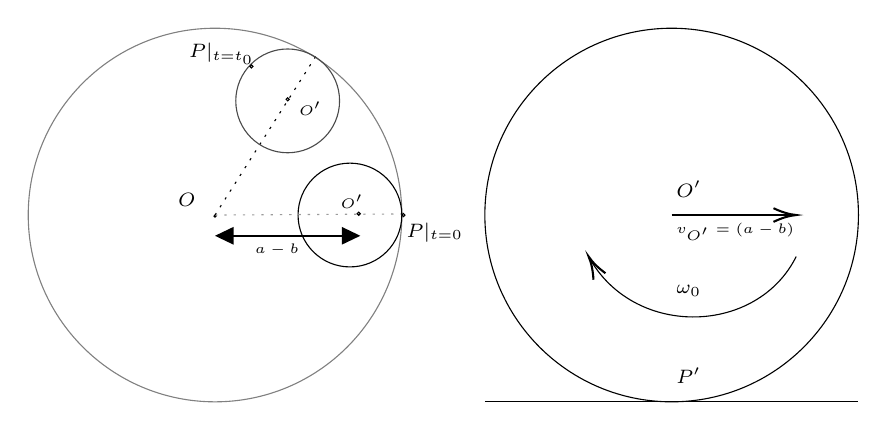
\begin{tikzpicture}[x=0.75pt,y=0.75pt,yscale=-1,xscale=1]
%uncomment if require: \path (0,300); %set diagram left start at 0, and has height of 300

%Shape: Circle [id:dp060733183983926464] 
\draw  [color={rgb, 255:red, 128; green, 128; blue, 128 }  ,draw opacity=1 ] (40,130) .. controls (40,80.29) and (80.29,40) .. (130,40) .. controls (179.71,40) and (220,80.29) .. (220,130) .. controls (220,179.71) and (179.71,220) .. (130,220) .. controls (80.29,220) and (40,179.71) .. (40,130) -- cycle ;
%Shape: Circle [id:dp7464527799159971] 
\draw   (129.5,130.5) .. controls (129.5,130.22) and (129.72,130) .. (130,130) .. controls (130.28,130) and (130.5,130.22) .. (130.5,130.5) .. controls (130.5,130.78) and (130.28,131) .. (130,131) .. controls (129.72,131) and (129.5,130.78) .. (129.5,130.5) -- cycle ;
%Shape: Circle [id:dp23294728589397795] 
\draw   (170,130) .. controls (170,116.19) and (181.19,105) .. (195,105) .. controls (208.81,105) and (220,116.19) .. (220,130) .. controls (220,143.81) and (208.81,155) .. (195,155) .. controls (181.19,155) and (170,143.81) .. (170,130) -- cycle ;
%Straight Lines [id:da6656257244146304] 
\draw [color={rgb, 255:red, 155; green, 155; blue, 155 }  ,draw opacity=1 ] [dash pattern={on 0.84pt off 2.51pt}]  (130,130) -- (219.5,129.5) ;
%Shape: Circle [id:dp8931660700101604] 
\draw   (200,129.35) .. controls (200,128.94) and (199.66,128.6) .. (199.25,128.6) .. controls (198.84,128.6) and (198.5,128.94) .. (198.5,129.35) .. controls (198.5,129.76) and (198.84,130.1) .. (199.25,130.1) .. controls (199.66,130.1) and (200,129.76) .. (200,129.35) -- cycle ;
%Straight Lines [id:da12357546116015339] 
\draw [line width=0.75]    (133,140) -- (197,140) ;
\draw [shift={(200,140)}, rotate = 180] [fill={rgb, 255:red, 0; green, 0; blue, 0 }  ][line width=0.08]  [draw opacity=0] (8.93,-4.29) -- (0,0) -- (8.93,4.29) -- cycle    ;
\draw [shift={(130,140)}, rotate = 0] [fill={rgb, 255:red, 0; green, 0; blue, 0 }  ][line width=0.08]  [draw opacity=0] (8.93,-4.29) -- (0,0) -- (8.93,4.29) -- cycle    ;
%Shape: Circle [id:dp013224691002791444] 
\draw   (221.5,130) .. controls (221.5,129.59) and (221.16,129.25) .. (220.75,129.25) .. controls (220.34,129.25) and (220,129.59) .. (220,130) .. controls (220,130.41) and (220.34,130.75) .. (220.75,130.75) .. controls (221.16,130.75) and (221.5,130.41) .. (221.5,130) -- cycle ;
%Straight Lines [id:da3091753982519425] 
\draw  [dash pattern={on 0.84pt off 2.51pt}]  (130,130) -- (179.4,52.2) ;
%Shape: Circle [id:dp4036251266953482] 
\draw  [color={rgb, 255:red, 74; green, 74; blue, 74 }  ,draw opacity=1 ] (140,75) .. controls (140,61.19) and (151.19,50) .. (165,50) .. controls (178.81,50) and (190,61.19) .. (190,75) .. controls (190,88.81) and (178.81,100) .. (165,100) .. controls (151.19,100) and (140,88.81) .. (140,75) -- cycle ;
%Shape: Circle [id:dp04106781309591723] 
\draw   (148.3,58.4) .. controls (148.3,57.99) and (147.96,57.65) .. (147.55,57.65) .. controls (147.14,57.65) and (146.8,57.99) .. (146.8,58.4) .. controls (146.8,58.81) and (147.14,59.15) .. (147.55,59.15) .. controls (147.96,59.15) and (148.3,58.81) .. (148.3,58.4) -- cycle ;
%Shape: Circle [id:dp3191860902024297] 
\draw   (165.75,74.25) .. controls (165.75,73.84) and (165.41,73.5) .. (165,73.5) .. controls (164.59,73.5) and (164.25,73.84) .. (164.25,74.25) .. controls (164.25,74.66) and (164.59,75) .. (165,75) .. controls (165.41,75) and (165.75,74.66) .. (165.75,74.25) -- cycle ;
%Straight Lines [id:da541108593951918] 
\draw    (260,220) -- (440,220) ;
%Shape: Circle [id:dp7750987114444706] 
\draw   (260,130) .. controls (260,80.29) and (300.29,40) .. (350,40) .. controls (399.71,40) and (440,80.29) .. (440,130) .. controls (440,179.71) and (399.71,220) .. (350,220) .. controls (300.29,220) and (260,179.71) .. (260,130) -- cycle ;
%Straight Lines [id:da08776229229255084] 
\draw    (350,130) -- (408,130) ;
\draw [shift={(410,130)}, rotate = 180] [color={rgb, 255:red, 0; green, 0; blue, 0 }  ][line width=0.75]    (10.93,-3.29) .. controls (6.95,-1.4) and (3.31,-0.3) .. (0,0) .. controls (3.31,0.3) and (6.95,1.4) .. (10.93,3.29)   ;
%Curve Lines [id:da34943197304242446] 
\draw    (310.99,151.75) .. controls (333.18,189.36) and (391.29,187.63) .. (410,150) ;
\draw [shift={(310,150)}, rotate = 61.49] [color={rgb, 255:red, 0; green, 0; blue, 0 }  ][line width=0.75]    (10.93,-3.29) .. controls (6.95,-1.4) and (3.31,-0.3) .. (0,0) .. controls (3.31,0.3) and (6.95,1.4) .. (10.93,3.29)   ;

% Text Node
\draw (111,118.4) node [anchor=north west][inner sep=0.75pt]  [font=\scriptsize]  {$O$};
% Text Node
\draw (189.2,119.2) node [anchor=north west][inner sep=0.75pt]  [font=\tiny]  {$O'$};
% Text Node
\draw (148,142.4) node [anchor=north west][inner sep=0.75pt]  [font=\tiny]  {$a-b$};
% Text Node
\draw (221,132.4) node [anchor=north west][inner sep=0.75pt]  [font=\scriptsize]  {$P|_{t=0}$};
% Text Node
\draw (116.2,46) node [anchor=north west][inner sep=0.75pt]  [font=\scriptsize]  {$P|_{t=t_{0}}$};
% Text Node
\draw (169.2,74.4) node [anchor=north west][inner sep=0.75pt]  [font=\tiny]  {$O'$};
% Text Node
\draw (351,112.4) node [anchor=north west][inner sep=0.75pt]  [font=\scriptsize]  {$O'$};
% Text Node
\draw (351,132.4) node [anchor=north west][inner sep=0.75pt]  [font=\tiny]  {$v_{O'} =( a-b) $};
% Text Node
\draw (351,202.4) node [anchor=north west][inner sep=0.75pt]  [font=\scriptsize]  {$P'$};
% Text Node
\draw (351,162.4) node [anchor=north west][inner sep=0.75pt]  [font=\scriptsize]  {$\omega _{0}$};


\end{tikzpicture}

    \end{center}
    \item This is similar to the problem above with a few changes. $O'$ now moves in a radius of $a+b$. The changed diagram is given below. Now we have $\omega_0=\frac{a+b}{b}$. The result follows.
    \begin{center}
        

\tikzset{every picture/.style={line width=0.75pt}} %set default line width to 0.75pt        

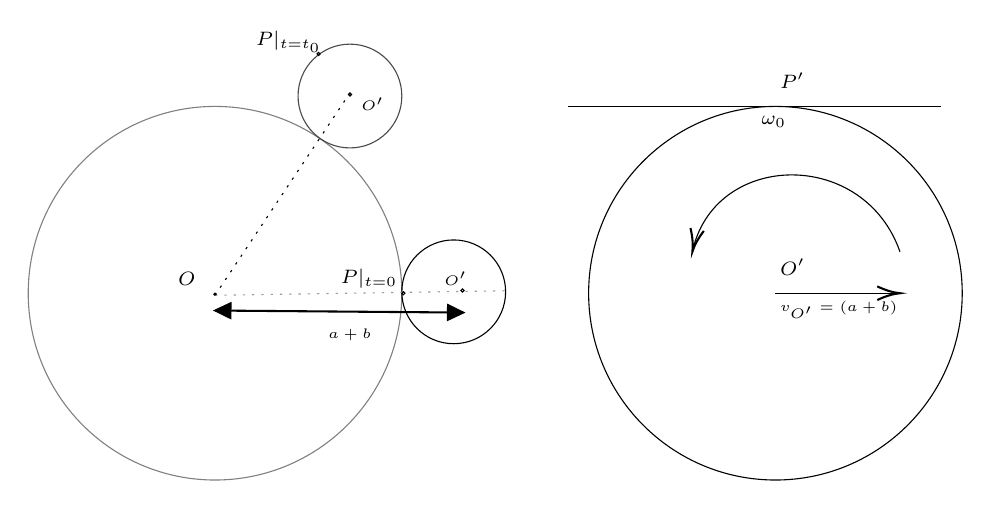
\begin{tikzpicture}[x=0.75pt,y=0.75pt,yscale=-1,xscale=1]
%uncomment if require: \path (0,300); %set diagram left start at 0, and has height of 300

%Shape: Circle [id:dp060733183983926464] 
\draw  [color={rgb, 255:red, 128; green, 128; blue, 128 }  ,draw opacity=1 ] (40,130) .. controls (40,80.29) and (80.29,40) .. (130,40) .. controls (179.71,40) and (220,80.29) .. (220,130) .. controls (220,179.71) and (179.71,220) .. (130,220) .. controls (80.29,220) and (40,179.71) .. (40,130) -- cycle ;
%Shape: Circle [id:dp7464527799159971] 
\draw   (129.5,130.5) .. controls (129.5,130.22) and (129.72,130) .. (130,130) .. controls (130.28,130) and (130.5,130.22) .. (130.5,130.5) .. controls (130.5,130.78) and (130.28,131) .. (130,131) .. controls (129.72,131) and (129.5,130.78) .. (129.5,130.5) -- cycle ;
%Shape: Circle [id:dp23294728589397795] 
\draw   (220,129.33) .. controls (220,115.53) and (231.19,104.33) .. (245,104.33) .. controls (258.81,104.33) and (270,115.53) .. (270,129.33) .. controls (270,143.14) and (258.81,154.33) .. (245,154.33) .. controls (231.19,154.33) and (220,143.14) .. (220,129.33) -- cycle ;
%Straight Lines [id:da6656257244146304] 
\draw [color={rgb, 255:red, 155; green, 155; blue, 155 }  ,draw opacity=1 ] [dash pattern={on 0.84pt off 2.51pt}]  (130,131) -- (269.5,128.83) ;
%Shape: Circle [id:dp8931660700101604] 
\draw   (250,128.68) .. controls (250,128.27) and (249.66,127.93) .. (249.25,127.93) .. controls (248.84,127.93) and (248.5,128.27) .. (248.5,128.68) .. controls (248.5,129.1) and (248.84,129.43) .. (249.25,129.43) .. controls (249.66,129.43) and (250,129.1) .. (250,128.68) -- cycle ;
%Straight Lines [id:da12357546116015339] 
\draw [line width=0.75]    (132,138.36) -- (247.67,139.31) ;
\draw [shift={(250.67,139.33)}, rotate = 180.47] [fill={rgb, 255:red, 0; green, 0; blue, 0 }  ][line width=0.08]  [draw opacity=0] (8.93,-4.29) -- (0,0) -- (8.93,4.29) -- cycle    ;
\draw [shift={(129,138.33)}, rotate = 0.47] [fill={rgb, 255:red, 0; green, 0; blue, 0 }  ][line width=0.08]  [draw opacity=0] (8.93,-4.29) -- (0,0) -- (8.93,4.29) -- cycle    ;
%Shape: Circle [id:dp013224691002791444] 
\draw   (221.5,130) .. controls (221.5,129.59) and (221.16,129.25) .. (220.75,129.25) .. controls (220.34,129.25) and (220,129.59) .. (220,130) .. controls (220,130.41) and (220.34,130.75) .. (220.75,130.75) .. controls (221.16,130.75) and (221.5,130.41) .. (221.5,130) -- cycle ;
%Straight Lines [id:da3091753982519425] 
\draw  [dash pattern={on 0.84pt off 2.51pt}]  (130,131) -- (195,33.5) ;
%Shape: Circle [id:dp4036251266953482] 
\draw  [color={rgb, 255:red, 74; green, 74; blue, 74 }  ,draw opacity=1 ] (170,35) .. controls (170,21.19) and (181.19,10) .. (195,10) .. controls (208.81,10) and (220,21.19) .. (220,35) .. controls (220,48.81) and (208.81,60) .. (195,60) .. controls (181.19,60) and (170,48.81) .. (170,35) -- cycle ;
%Shape: Circle [id:dp04106781309591723] 
\draw   (180.63,14.73) .. controls (180.63,14.32) and (180.3,13.98) .. (179.88,13.98) .. controls (179.47,13.98) and (179.13,14.32) .. (179.13,14.73) .. controls (179.13,15.15) and (179.47,15.48) .. (179.88,15.48) .. controls (180.3,15.48) and (180.63,15.15) .. (180.63,14.73) -- cycle ;
%Shape: Circle [id:dp3191860902024297] 
\draw   (195.75,34.25) .. controls (195.75,33.84) and (195.41,33.5) .. (195,33.5) .. controls (194.59,33.5) and (194.25,33.84) .. (194.25,34.25) .. controls (194.25,34.66) and (194.59,35) .. (195,35) .. controls (195.41,35) and (195.75,34.66) .. (195.75,34.25) -- cycle ;
%Straight Lines [id:da541108593951918] 
\draw    (300,40) -- (480,40) ;
%Shape: Circle [id:dp7750987114444706] 
\draw   (310,130) .. controls (310,80.29) and (350.29,40) .. (400,40) .. controls (449.71,40) and (490,80.29) .. (490,130) .. controls (490,179.71) and (449.71,220) .. (400,220) .. controls (350.29,220) and (310,179.71) .. (310,130) -- cycle ;
%Straight Lines [id:da08776229229255084] 
\draw    (400,130) -- (458,130) ;
\draw [shift={(460,130)}, rotate = 180] [color={rgb, 255:red, 0; green, 0; blue, 0 }  ][line width=0.75]    (10.93,-3.29) .. controls (6.95,-1.4) and (3.31,-0.3) .. (0,0) .. controls (3.31,0.3) and (6.95,1.4) .. (10.93,3.29)   ;
%Curve Lines [id:da34943197304242446] 
\draw    (360.51,107.86) .. controls (372.48,61.62) and (442.6,60.42) .. (460,110) ;
\draw [shift={(360,110)}, rotate = 282.07] [color={rgb, 255:red, 0; green, 0; blue, 0 }  ][line width=0.75]    (10.93,-3.29) .. controls (6.95,-1.4) and (3.31,-0.3) .. (0,0) .. controls (3.31,0.3) and (6.95,1.4) .. (10.93,3.29)   ;

% Text Node
\draw (111,118.4) node [anchor=north west][inner sep=0.75pt]  [font=\scriptsize]  {$O$};
% Text Node
\draw (239.2,118.53) node [anchor=north west][inner sep=0.75pt]  [font=\tiny]  {$O'$};
% Text Node
\draw (183.33,145.73) node [anchor=north west][inner sep=0.75pt]  [font=\tiny]  {$a+b$};
% Text Node
\draw (189.33,117.07) node [anchor=north west][inner sep=0.75pt]  [font=\scriptsize]  {$P|_{t=0}$};
% Text Node
\draw (148.53,2.33) node [anchor=north west][inner sep=0.75pt]  [font=\scriptsize]  {$P|_{t=t_{0}}$};
% Text Node
\draw (199.2,34.4) node [anchor=north west][inner sep=0.75pt]  [font=\tiny]  {$O'$};
% Text Node
\draw (401,112.4) node [anchor=north west][inner sep=0.75pt]  [font=\scriptsize]  {$O'$};
% Text Node
\draw (401,132.4) node [anchor=north west][inner sep=0.75pt]  [font=\tiny]  {$v_{O'} =( a+b)$};
% Text Node
\draw (401,22.4) node [anchor=north west][inner sep=0.75pt]  [font=\scriptsize]  {$P'$};
% Text Node
\draw (392,43.4) node [anchor=north west][inner sep=0.75pt]  [font=\scriptsize]  {$\omega _{0}$};


\end{tikzpicture}

    \end{center}
    \item $P$ has zero velocity if and only if it is in contact with $C'$, in which case it forms a cusp. Therefore, whenever $\gamma$ is smooth, it is regular.
    \item If $m=1$ then $P$ touches $C'$ at only one point. The result follows.
    \item If $m=1/4$ then $P$ touches $C'$at $4$ points. The result follows.
    \item Let the curve reach it's starting point at $t=t_0$. Then $O'(0)=O'(t_o)$. Therefore, $t_0=2q\pi$ where $q\in\mathbb N$. We also want the smaller circle to make a integral number of rotations during this time. Now, the angular velocity of the smaller circle is $(1/m\pm 1)$(sign depending on if curve is hypocycloid or epicycloid).We therefore have: $(1/m\pm 1)q2\pi=p2\pi$ which on simplification gives
    $m=\frac{1}{p/q\pm 1}$ which is a rational number.
\end{enumerate}

\subsection{Problem 3}\textbf{
Snowy has been very naughty, forcing Tintin (in the rarest of rare circumstances) to put him on a leash
of length 1 unit. No sooner did Snowy finish burying a bone at (0, 1) that Tintin began to take a walk in Marlinspike along the x-axis (in the positive direction), starting at the origin. Captain Haddock was accompanying Tintin on his
walk. As natural instincts guided Snowy to get back to the bone, he always pulled the leash taut while he was being
dragged by Tintin. The curve traced out by Snowy is the \textit{tractrix}. Note that Snowy pulling the leash taut simply
means that the leash will be tangent to the curve.
\begin{figure}
    \centering
    \includegraphics[width=0.3\textwidth]{snowy.png}
    \includegraphics[width=0.3\textwidth]{tintin.png}
    \caption{a. Snowy before burying the unusually large bone b. Tintin and Captain taking a walk}
    \label{fig:my_label}
\end{figure}
\begin{enumerate}
    \item Graph the tractrix.
    \item Show that $\alpha(\theta)=(\cos\theta+\ln\tan\frac{\theta}{2},\sin\theta$ is a prameterization in terms of the angle the tangent makes with the x-axis.
    \item Show that $\gamma(t)=(t-\tanh t,\sech t)$ for $t\geq0$ is another parameterization of the tactrix.
\end{enumerate}}
\textbf{Solutions:}
\begin{figure}
    \centering
    \includegraphics[width=0.4\textwidth]{Tractrix.png}
    \caption{3.1 Tractrix. Copied shamelessly from wikipedia. For our problem, the trace will be horizontal rather than vertical and only the portion to the right of x-axis will be present.}
    \label{fig:my_label}
\end{figure}
\begin{enumerate}[start=2]
    \item Note that $\alpha'(\theta)=(1/\sin\theta-\sin\theta,\cos\theta)$ and $m(\theta)=\tan\theta$ as expected.\\
    Consider the point where tintin is at when the rope makes a slope of $\tan\theta$. Let he be at $(x,0)$.Then $(x-\cos\theta-\ln\tan(\theta/2)-\cos\theta)^2+\sin^2\theta=1$. Then $x=2\cos\theta+\ln\tan\theta/2$. Then as required, this point makes an angle $\theta$ with $\alpha\theta$ and therefor lies on the tangent.
    \item Same as above.
\end{enumerate}

\subsection{Problem 4}\textbf{Suppose $\alpha:[a,b]\to\mathbb R^2$ is a smooth parametrized plane curve. Prove that if the chord length
$||\alpha(t_1)-\alpha(t_2)||$ depends only on $|t_1-t_2|$ then $\alpha$ must be a (subset of) a line or a circle.\\\\
Solution:}\\


\subsection{Problem 5}\textbf{This problem involves the catenary.
\begin{enumerate}
    \item Show that the arc-length of the catenary $\gamma(t) = (t, \cosh t)$ for $0 \leq  t \leq b $ is $\sinh b$.
    \item Reparametrize the catenary by arc-length.
    \item Recall the curve obtained in order to ride a bicycle with square wheels smoothly. Show that it is built out of
inverted catenaries.
\end{enumerate}
Solution:}
\begin{enumerate}
    \item We have
    \begin{align*}
        \gamma(t)=\left(t,\cosh (t)\right)\quad \gamma'(t)=\left(1,\sinh(t)\right)\quad||\gamma'(t)||=\sqrt{\left(1+\frac{e^{2x}+e^{-2x}-2}{4}\right)}&=\sqrt{\left(\frac{e^{2x}+e^{-2x}+2}{4}\right)}=\cosh(t)
    \end{align*}
    It follows curve length is:
    $$S(b)=\int_0^b\cosh(t)dt=\int_0^b\frac{e^{t}+e^{-t}}{2}dt=\frac{e^{b}+e^{-b}}{2}=\sinh(b)$$
    \item Let $\varphi(t)=S^{-1}(t)=\sinh^{-1}(t)=
    \ln(t+\sqrt{t^2-1})$(to get the last identity, set $e^{t}=u$ in $\cosh (t)=\frac{e^{2t}+1}{2e^t}$ and solve the quadratic). Then reprameterization is given by:
    $$\eta=\gamma\circ\varphi(t)=
    \left(\ln(t+\sqrt{t^2-1}),(t^2-1+\sqrt{t^2-1})\right) $$
    \item The assumptions we take are:
    \begin{enumerate}
        \item The center of the wheel is at a constant elevation
        \item The point of contact is always below the center
    \end{enumerate}
    \begin{center}
        

\tikzset{every picture/.style={line width=0.75pt}} %set default line width to 0.75pt        

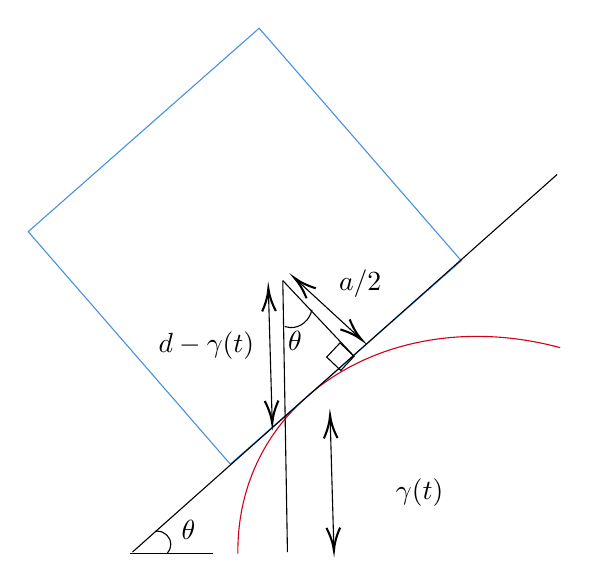
\begin{tikzpicture}[x=0.75pt,y=0.75pt,yscale=-1,xscale=1]
%uncomment if require: \path (0,300); %set diagram left start at 0, and has height of 300

%Curve Lines [id:da06483635235223006] 
\draw [color={rgb, 255:red, 208; green, 2; blue, 27 }  ,draw opacity=1 ]   (194.13,271) .. controls (193.38,195.84) and (268.78,150) .. (349.4,171.79) ;
%Shape: Rectangle [id:dp6764089345376411] 
\draw  [color={rgb, 255:red, 74; green, 144; blue, 226 }  ,draw opacity=1 ] (93.12,115.91) -- (204.38,17.89) -- (301.75,129.9) -- (190.49,227.93) -- cycle ;
%Straight Lines [id:da6160193174149843] 
\draw    (143.36,270.25) -- (347.91,88.37) ;
%Straight Lines [id:da8967183974203027] 
\draw    (142.2,271) -- (182.2,271) ;
%Shape: Arc [id:dp6204720319414534] 
\draw  [draw opacity=0] (154.15,260.3) .. controls (154.52,260.23) and (154.91,260.2) .. (155.3,260.2) .. controls (158.89,260.2) and (161.8,263.07) .. (161.8,266.6) .. controls (161.8,268.27) and (161.15,269.79) .. (160.09,270.93) -- (155.3,266.6) -- cycle ; \draw   (154.15,260.3) .. controls (154.52,260.23) and (154.91,260.2) .. (155.3,260.2) .. controls (158.89,260.2) and (161.8,263.07) .. (161.8,266.6) .. controls (161.8,268.27) and (161.15,269.79) .. (160.09,270.93) ;  
%Straight Lines [id:da3749744165815425] 
\draw    (215.77,139.48) -- (250.11,175.94) ;
%Straight Lines [id:da10203198279226555] 
\draw    (215.77,139.48) -- (218.01,270.25) ;
%Shape: Rectangle [id:dp1446353278473238] 
\draw   (236.92,176.33) -- (243.33,169.5) -- (250.11,175.94) -- (243.71,182.78) -- cycle ;
%Shape: Arc [id:dp6717429242107007] 
\draw  [draw opacity=0] (229.83,153.59) .. controls (228.64,158.7) and (224.27,162.37) .. (219.28,162.11) .. controls (218.39,162.06) and (217.53,161.89) .. (216.71,161.62) -- (219.85,150.9) -- cycle ; \draw   (229.83,153.59) .. controls (228.64,158.7) and (224.27,162.37) .. (219.28,162.11) .. controls (218.39,162.06) and (217.53,161.89) .. (216.71,161.62) ;  
%Straight Lines [id:da3022104244061832] 
\draw    (238.6,206.49) -- (240.35,267.5) ;
\draw [shift={(240.41,269.5)}, rotate = 268.36] [color={rgb, 255:red, 0; green, 0; blue, 0 }  ][line width=0.75]    (10.93,-3.29) .. controls (6.95,-1.4) and (3.31,-0.3) .. (0,0) .. controls (3.31,0.3) and (6.95,1.4) .. (10.93,3.29)   ;
\draw [shift={(238.54,204.49)}, rotate = 88.36] [color={rgb, 255:red, 0; green, 0; blue, 0 }  ][line width=0.75]    (10.93,-3.29) .. controls (6.95,-1.4) and (3.31,-0.3) .. (0,0) .. controls (3.31,0.3) and (6.95,1.4) .. (10.93,3.29)   ;
%Straight Lines [id:da7161120526604502] 
\draw    (208.87,145.31) -- (210.63,206.32) ;
\draw [shift={(210.68,208.32)}, rotate = 268.36] [color={rgb, 255:red, 0; green, 0; blue, 0 }  ][line width=0.75]    (10.93,-3.29) .. controls (6.95,-1.4) and (3.31,-0.3) .. (0,0) .. controls (3.31,0.3) and (6.95,1.4) .. (10.93,3.29)   ;
\draw [shift={(208.82,143.31)}, rotate = 88.36] [color={rgb, 255:red, 0; green, 0; blue, 0 }  ][line width=0.75]    (10.93,-3.29) .. controls (6.95,-1.4) and (3.31,-0.3) .. (0,0) .. controls (3.31,0.3) and (6.95,1.4) .. (10.93,3.29)   ;
%Straight Lines [id:da9859574606139355] 
\draw    (222.87,139.55) -- (252.33,166.65) ;
\draw [shift={(253.8,168)}, rotate = 222.61] [color={rgb, 255:red, 0; green, 0; blue, 0 }  ][line width=0.75]    (10.93,-3.29) .. controls (6.95,-1.4) and (3.31,-0.3) .. (0,0) .. controls (3.31,0.3) and (6.95,1.4) .. (10.93,3.29)   ;
\draw [shift={(221.4,138.2)}, rotate = 42.61] [color={rgb, 255:red, 0; green, 0; blue, 0 }  ][line width=0.75]    (10.93,-3.29) .. controls (6.95,-1.4) and (3.31,-0.3) .. (0,0) .. controls (3.31,0.3) and (6.95,1.4) .. (10.93,3.29)   ;

% Text Node
\draw (165.79,253.48) node [anchor=north west][inner sep=0.75pt]    {$\theta $};
% Text Node
\draw (217.11,162.43) node [anchor=north west][inner sep=0.75pt]    {$\theta $};
% Text Node
\draw (269.02,233.71) node [anchor=north west][inner sep=0.75pt]    {$\gamma ( t)$};
% Text Node
\draw (154.66,162.76) node [anchor=north west][inner sep=0.75pt]    {$d-\gamma ( t)$};
% Text Node
\draw (241.6,133) node [anchor=north west][inner sep=0.75pt]    {$a/2$};


\end{tikzpicture}

    \end{center}
    We note the figure given above. Note: $\tan\theta=\gamma'(t)$ and $\cos\theta =\frac{a/2}{d-\gamma'(t)}$. The differential equation is therefore given by:
    $$\sqrt{1+\gamma'(t)^2}=\frac{d-\gamma(t)}{a/2}$$
\end{enumerate}
The solution to which is a inverted catenary.


\section{Homework 3}

\subsection{This question concerns the Inverse Function Theorem in one variable.
}\textbf{
\begin{enumerate}
\item  Let $f : (\alpha, \beta)\to\mathbb R$ be a smooth function such that $f'$
is nowhere zero. Note that $-\infty \leq \alpha < \beta \leq \infty$.
\begin{enumerate}
    \item Show that the image is path-connected.
    \item Show that the image is an open set. Hence, or otherwise, conclude that image of $f$ is $(\alpha',\beta')$, where 
    $$\alpha'=\lim_{t\to \alpha^+}f(t)\quad \beta'=\lim_{t\to \beta^-}f(t)$$ 
    Note that $\alpha'$ can be $-\infty$ and $\beta'$ can be $\infty$. 
    \item Show that $f:(\alpha,\beta)\to (\alpha',\beta')$ is a monotonic bijection.
    \item Let $g$ be the inverse of $f$. Show that $g$ is of class $C^1$ by showing that its linearization is given by:
    $g'(t)=\left(f'\circ g(t)\right)^{-1}$ 
    [You have to show this; a mere formal computation/differentiation is not satisfactory!]
\end{enumerate} 
\item  (Inverse Function Theorem) Let $f : (\alpha, \beta) \to\mathbb R$ be a smooth map such that $f'(a)\ne 0$ for some $a\in(\alpha,\beta)$. Show
that there exists open neighbourhoods $U$ of $a$ and $V$ of $f(a)$ such that $f : U \to V$ is a diffeomorphism. \textit{[Part (1) will
be useful.]}
\end{enumerate}}
\textbf{Solution :}
\begin{enumerate}
    \item Let the image be not path connected. Therefore, there exists $c$ such that $c$ lies between $f(\alpha)$ and $f(\beta)$ such that $c\notin \left(f(\alpha,)f(\beta)\right)$. But this leads to a contradiction due to intermediate value theorem. \\
    Let $f$ be non monotonic and $\alpha<c<\beta$. Let $f(c)>f(\alpha)\geq f(\beta)$. Then there exist $p$ between $c$ and $\beta$ such that $f(p)=f(a)$. If we apply LMVT then we get $p'$ between $\alpha$ and $p$ such that $f'(p')=0$ leading to a contradiction.
    \begin{center}
        

\tikzset{every picture/.style={line width=0.75pt}} %set default line width to 0.75pt        

\begin{tikzpicture}[x=0.75pt,y=0.75pt,yscale=-1,xscale=1]
%uncomment if require: \path (0,300); %set diagram left start at 0, and has height of 300

%Straight Lines [id:da8967183974203027] 
\draw    (142.2,271) -- (182.2,271) ;
%Shape: Circle [id:dp9204741670063893] 
\draw  [fill={rgb, 255:red, 0; green, 0; blue, 0 }  ,fill opacity=1 ] (99.2,104.6) .. controls (99.2,101.62) and (101.62,99.2) .. (104.6,99.2) .. controls (107.58,99.2) and (110,101.62) .. (110,104.6) .. controls (110,107.58) and (107.58,110) .. (104.6,110) .. controls (101.62,110) and (99.2,107.58) .. (99.2,104.6) -- cycle ;
%Shape: Circle [id:dp5525179626222491] 
\draw  [fill={rgb, 255:red, 0; green, 0; blue, 0 }  ,fill opacity=1 ] (319.2,154.6) .. controls (319.2,151.62) and (321.62,149.2) .. (324.6,149.2) .. controls (327.58,149.2) and (330,151.62) .. (330,154.6) .. controls (330,157.58) and (327.58,160) .. (324.6,160) .. controls (321.62,160) and (319.2,157.58) .. (319.2,154.6) -- cycle ;
%Shape: Circle [id:dp9864224484874724] 
\draw  [fill={rgb, 255:red, 0; green, 0; blue, 0 }  ,fill opacity=1 ] (219.2,44.6) .. controls (219.2,41.62) and (221.62,39.2) .. (224.6,39.2) .. controls (227.58,39.2) and (230,41.62) .. (230,44.6) .. controls (230,47.58) and (227.58,50) .. (224.6,50) .. controls (221.62,50) and (219.2,47.58) .. (219.2,44.6) -- cycle ;
%Curve Lines [id:da8739540629167332] 
\draw    (140,60) .. controls (171.8,28.2) and (209,23.4) .. (240,60) ;
%Straight Lines [id:da3395794591547585] 
\draw  [dash pattern={on 0.84pt off 2.51pt}]  (110,90) -- (130,70) ;
%Straight Lines [id:da6404348108645128] 
\draw  [dash pattern={on 0.84pt off 2.51pt}]  (324.6,154.6) -- (300,130) ;
%Shape: Circle [id:dp7122759578985809] 
\draw  [fill={rgb, 255:red, 0; green, 0; blue, 0 }  ,fill opacity=1 ] (274.2,105.4) .. controls (274.2,102.42) and (276.62,100) .. (279.6,100) .. controls (282.58,100) and (285,102.42) .. (285,105.4) .. controls (285,108.38) and (282.58,110.8) .. (279.6,110.8) .. controls (276.62,110.8) and (274.2,108.38) .. (274.2,105.4) -- cycle ;
%Straight Lines [id:da8636240094814364] 
\draw    (268.1,93.9) -- (291.1,116.9) ;

% Text Node
\draw (111,92.4) node [anchor=north west][inner sep=0.75pt]    {$f( \alpha )$};
% Text Node
\draw (331,142.4) node [anchor=north west][inner sep=0.75pt]    {$f( \beta )$};
% Text Node
\draw (231,32.4) node [anchor=north west][inner sep=0.75pt]    {$f( c)$};
% Text Node
\draw (287.2,91.4) node [anchor=north west][inner sep=0.75pt]    {$f( p)$};


\end{tikzpicture}

    \end{center}
    This is not the only case. The order of $f(\alpha)$ and $f(\beta)$ can be different and there might be a minima instead of maxima but the proof stays almost same. Therefore, $f$ is monotonic and bijection with it's image. For part 2 we need to assume $f$ is increasing. Let $c\in(f(\alpha),f(\beta))$. Then $c=f(y)$ for some $y$. Set $\alpha'=\frac{\alpha+y}{2}$, $\beta'=\frac{\beta+y}{2}$. Then $(f(\alpha'),f(\beta'))$ is an open neighbourhood around $c$. Therefore, the image is a open set. Now as the image set is open and connected it is of the form $(\alpha',\beta')$. Then $(b)$ and $(c)$ follows. $d$ follows from first principles.
\item $f'$ follows intermediate value theorem. Therefore, there exist some open neighbourhood around $a$ where the conditions of $1$ is satisfied. The result follows. 
\end{enumerate}
\textbf{Alt sol of part(c):} As $f'\ne0$ and $f'$ follows the intermediate value theorem, $f'$ doesn't change signs in the range.  Therefore, $f$ is monotonic.























\twocolumn















































\chapter{Appendix}
\section{Some specific curves taught in class}
\subsection{Parabola}




\section{Differentiability of curves}
\begin{definition}[Differentiable function]
A continuous function $f:(a,b)\to\mathbb R$(\textit{Note:} $a,b$ might be $\pm \infty$, in which case the function is defined on whole of $\mathbb R$) is called differentiable or of type $c^1$ if $$f'(x)=\lim_{h\to 0}\frac{f(x+h)-f(x)}{h}$$
exists and is continuous.
\end{definition}
In a similar way, we can define $C^2,C^3$ and  $C^k$ by differentiating $f$ $2,3,k$ times respectively. We call a function ``\textit{smooth}'' if the function is $C^k$ for any $k\in\mathbb N$.\\
\textbf{Examples}
\begin{enumerate}
    \item $f(x)=|x|$: This is a $C^0$ function as $f$ is not differentiable at 0.
    \item $$f(x)=\begin{cases}x^2\sin\left(\frac{1}{x}\right)\quad&x\ne0\\
    0\quad&x=0
    \end{cases}$$
    $f'$ exists but is not continuous. So $f'$ is not continuous. 
\end{enumerate}
\section{Differentiation (Multivariable)}
\begin{definition}[Differentiable multivariable function]
A function $f:(a,b)\to\mathbb R$ is of class $C^k$ if every $\pi_i\circ f(x)$ is $C^k$ where $\pi_i$ is projection to the $i^{th}$ coordinate.
\end{definition}
\textbf{Notation:} We define $$\nabla_vf(p)=\lim_{t\to 0}\frac{f(p+tv)-f(p)}{t} $$\\
For $C^1$ functions let $v=v_1+v_2$. Then:
\begin{align*}
    \nabla_vf(p)-\nabla_{v_1}f(p)&=\lim_{t\to0}\frac{f(p+tv_1+tv_2)-f(p+tv_1)}{t}\\
    &=\lim_{t\to0}\nabla_{v_2}f(p+tv_1)=\nabla_{v_2}f(p) 
\end{align*}
\begin{align*}
    \nabla_{kv}f(p)&=\lim_{t\to0}\frac{f(p+tkv)-f(p)}{t}\\
    &=k\lim_{t\to0}\frac{f(p+tkv)-f(p)}{kt}\\
    &=k\nabla_vf(p)    
\end{align*}
If $v=\sum_{i=1}^nc_ie_i$, then we can apply the above formula repeatedly to get   $\nabla_vf(p)=\sum_{i=1}^nc_i\nabla_{e_i}f(p)$.
\begin{definition}[Differentiation of multivariable function]
A function $\mathbb R^n\to\mathbb R^m$ is differntiable at $a$ if there exists a linear map $L_a:\mathbb R^n\to\mathbb R^m$ such that
$$f(a+v)-f(a)-L_a(v)=E_a(v)||v||$$
where $\lim_{v\to 0}E_a(v)=0$.
\end{definition}
A function $f$ is called differntiable if such a linear map exists and $D_f(a)=L_a$. We can define a map $\Tilde{D_f}:\mathbb R^n\times\mathbb R^m\to\mathbb R^m,\Tilde{D_f}(a,v)=L_av$. This map is studied in differential geometry. 
%%Need to prove D_f is cts iff \tilde D_f is cts.
A nice condition is if all the $k^{th}$ derivative $\frac{\partial^k}{\partial x_i^{k_i}}f,\sum k_i=k$ exits and is continuous then $f$ is $C^k$ continuous. 
\section{Homeomorphism, Diffeomorphism and invariance of domain}
\begin{definition}[Diffeomorphism]
Let $U\in\mathbb R^n$ and $V\in\mathbb R^m$ be open sets of $\mathbb R^n$ and $\mathbb R^m$ repectively. A map $f:U\to V$ is a diffeomorphism if $f$ is $C^\infty$ and if $f$ has a smooth inverse.
\end{definition}
If we consider homeomorphism between $U,V$ then it is required that $m=n$. This proof requires techniques of algebric topology and is not discussed here.This is known as invariance of domain. But if we consider difeomorphisms, then we can prove $m=n$.
\begin{lemma}
Let $f:\mathbb R^l\to\mathbb R^m$ and $g:\mathbb R^m\to\mathbb R^n$ are smooth function then $f\circ g$ is smooth. 
\end{lemma}
\textbf{Notation: }We shall look at a nice way to write the differentiation operator. We say
$$Df(a,v)=D_f(a)v$$
For example, we shall write the chain rule as
$$D(g\circ f)(\overrightarrow{a},\overrightarrow{v})=Dg(f(\overrightarrow{a}),Df(\overrightarrow{a},\overrightarrow{v}))$$
\begin{corollary}
If there exists a difeeomorphism between $U\in\mathbb R^n$ and $V\in\mathbb R^m$ then $m=n$.
\end{corollary}
\begin{proof}
Without loss of generality, let $m\geq n$. Let $f:U\to V$ be the diffeomorphism and let $g$ be it's inverse. Then $D(f\circ g)(\overrightarrow{a},\cdot)=D(Id_{m\times m})(\overrightarrow{a},\cdot)=Id_{m\times m}$. This follows because differentiation of a linear map $T$ is $T$ itself. But we also have
$$D(f\circ g)(\overrightarrow{a},\cdot)=Dg(f(\overrightarrow{a}),Df(\overrightarrow{a},\cdot))$$
Let $D_g(f(a))=L_{m}^n$ and $D_f(a)=L_{n}^m$. Therefore:
$$D(f\circ g)(\overrightarrow{a},v)=L_{n}^mL_m^nv$$
Now we use the rank nullity theorem. 
\begin{align*}
    dim(null(L_{m}^n))&=dim \mathbb{R}^m-dim(range(L_{m}^n))\\
    &\geq m-dim(\mathbb R^n)=m-n
\end{align*}
Now if $dim(null(L_{m}^n))\ne 0$ then we can get $v\ne 0$ such that $L_{n}^mL_m^nv=L_{n}^m0=0$. But this shouldn't happen as $L_{n}^mL_m^nv=Id_{m\times m}v=v$. So we need $m-n=0\Rightarrow m=n$.
\end{proof}
\textit{Note:} Our instructor gave a slight variation of the proof: he mentioned $L_{n}^mL_m^nv$ and $L_m^nvL_{n}^m$ can't be both invertible if $m\ne n$. I felt what he said was trivial but still need to be written out.





\end{document}
